%%%%%%%% ICML 2026 EXAMPLE LATEX SUBMISSION FILE %%%%%%%%%%%%%%%%%

\documentclass{article}

% Recommended, but optional, packages for figures and better typesetting:
\usepackage{microtype}
\usepackage{graphicx}
\usepackage{subcaption}
\usepackage{booktabs} % for professional tables

% hyperref makes hyperlinks in the resulting PDF.
% If your build breaks (sometimes temporarily if a hyperlink spans a page)
% please comment out the following usepackage line and replace
% \usepackage{icml2026} with \usepackage[nohyperref]{icml2026} above.
\usepackage{hyperref}


% Attempt to make hyperref and algorithmic work together better:
\newcommand{\theHalgorithm}{\arabic{algorithm}}

% Use the following line for the initial blind version submitted for review:
\usepackage{icml2026}

% For preprint, use
% \usepackage[preprint]{icml2026}

% If accepted, instead use the following line for the camera-ready submission:
% \usepackage[accepted]{icml2026}

\usepackage{amsmath, amssymb, amsthm}
\usepackage{algorithm}
\usepackage{algorithmic}
\usepackage{graphicx}
\graphicspath{{figures/}{results/}}
\usepackage{booktabs}
\usepackage{multirow}
%\usepackage[colorlinks=true, linkcolor=blue, citecolor=green]{hyperref}
\usepackage[capitalize,noabbrev]{cleveref}
\usepackage{bm}
\usepackage{cases}

\DeclareMathOperator*{\argmin}{arg\,min}
\DeclareMathOperator*{\argmax}{arg\,max}

\newcommand{\R}{\mathbb{R}}
\newcommand{\E}{\mathbb{E}}
\newcommand{\var}{\text{Var}}
\newcommand{\trans}{^{\top}}
\newcommand{\norm}[1]{\lVert #1 \rVert}
\newcommand{\abs}[1]{\lvert #1 \rvert}
\newcommand{\inner}[2]{\langle #1, #2 \rangle}
\newcommand{\diag}{\text{diag}}
\newcommand{\sign}{\text{sign}}

\theoremstyle{plain}
\newtheorem{theorem}{Theorem}
\newtheorem{lemma}{Lemma}
\newtheorem{corollary}{Corollary}
\newtheorem{proposition}{Proposition}
\theoremstyle{definition}
\newtheorem{definition}{Definition}
\theoremstyle{remark}
\newtheorem{remark}{Remark}
\newtheorem{assumption}{Assumption}

%\usepackage{amsmath}
%\usepackage{amssymb}
%\usepackage{mathtools}
%\usepackage{amsthm}
%
%\DeclareMathOperator*{\argmin}{arg\,min}
%
%
%% if you use cleveref..
%\usepackage[capitalize,noabbrev]{cleveref}
%
%%%%%%%%%%%%%%%%%%%%%%%%%%%%%%%%%
%% THEOREMS
%%%%%%%%%%%%%%%%%%%%%%%%%%%%%%%%%
%\theoremstyle{plain}
%\newtheorem{theorem}{Theorem}[section]
%\newtheorem{proposition}[theorem]{Proposition}
%\newtheorem{lemma}[theorem]{Lemma}
%\newtheorem{corollary}[theorem]{Corollary}
%\theoremstyle{definition}
%\newtheorem{definition}[theorem]{Definition}
%\newtheorem{assumption}[theorem]{Assumption}
%\theoremstyle{remark}
%\newtheorem{remark}[theorem]{Remark}
%
%\usepackage{bm}
%
%\newcommand{\R}{\mathbb{R}}
%\newcommand{\E}{\mathbb{E}}
%\newcommand{\var}{\text{Var}}
%\newcommand{\trans}{^{\top}}
%\newcommand{\norm}[1]{\lVert #1 \rVert}
%% 在导言区添加这些定义
%\DeclareMathOperator{\softmax}{softmax}

% Todonotes is useful during development; simply uncomment the next line
%    and comment out the line below the next line to turn off comments
%\usepackage[disable,textsize=tiny]{todonotes}
\usepackage[textsize=tiny]{todonotes}

% The \icmltitle you define below is probably too long as a header.
% Therefore, a short form for the running title is supplied here:
\icmltitlerunning{Submission and Formatting Instructions for ICML 2026}

\begin{document}

\twocolumn[
  \icmltitle{Implicit Regularization in Nonlinear In-Context Learning}

  % It is OKAY to include author information, even for blind submissions: the
  % style file will automatically remove it for you unless you've provided
  % the [accepted] option to the icml2026 package.

  % List of affiliations: The first argument should be a (short) identifier you
  % will use later to specify author affiliations Academic affiliations
  % should list Department, University, City, Region, Country Industry
  % affiliations should list Company, City, Region, Country

  % You can specify symbols, otherwise they are numbered in order. Ideally, you
  % should not use this facility. Affiliations will be numbered in order of
  % appearance and this is the preferred way.
  \icmlsetsymbol{equal}{*}

  \begin{icmlauthorlist}
    \icmlauthor{Firstname1 Lastname1}{equal,yyy}
    \icmlauthor{Firstname2 Lastname2}{equal,yyy,comp}
    \icmlauthor{Firstname3 Lastname3}{comp}
    \icmlauthor{Firstname4 Lastname4}{sch}
    \icmlauthor{Firstname5 Lastname5}{yyy}
    \icmlauthor{Firstname6 Lastname6}{sch,yyy,comp}
    \icmlauthor{Firstname7 Lastname7}{comp}
    %\icmlauthor{}{sch}
    \icmlauthor{Firstname8 Lastname8}{sch}
    \icmlauthor{Firstname8 Lastname8}{yyy,comp}
    %\icmlauthor{}{sch}
    %\icmlauthor{}{sch}
  \end{icmlauthorlist}

  \icmlaffiliation{yyy}{Department of XXX, University of YYY, Location, Country}
  \icmlaffiliation{comp}{Company Name, Location, Country}
  \icmlaffiliation{sch}{School of ZZZ, Institute of WWW, Location, Country}

  \icmlcorrespondingauthor{Firstname1 Lastname1}{first1.last1@xxx.edu}
  \icmlcorrespondingauthor{Firstname2 Lastname2}{first2.last2@www.uk}

  % You may provide any keywords that you find helpful for describing your
  % paper; these are used to populate the "keywords" metadata in the PDF but
  % will not be shown in the document
  \icmlkeywords{Machine Learning, ICML}

  \vskip 0.3in
]

% this must go after the closing bracket ] following \twocolumn[ ...

% This command actually creates the footnote in the first column listing the
% affiliations and the copyright notice. The command takes one argument, which
% is text to display at the start of the footnote. The \icmlEqualContribution
% command is standard text for equal contribution. Remove it (just {}) if you
% do not need this facility.

% Use ONE of the following lines. DO NOT remove the command.
% If you have no special notice, KEEP empty braces:
\printAffiliationsAndNotice{}  % no special notice (required even if empty)
% Or, if applicable, use the standard equal contribution text:
% \printAffiliationsAndNotice{\icmlEqualContribution}

\begin{abstract}
	
Recent theoretical advances have established that linear transformers perform in-context learning (ICL) by implementing gradient descent on linear regression tasks, often equivalent to ridge regression. However, real-world language models employ nonlinear activations (e.g., ReLU, GeLU) and softmax attention, whose implicit regularization effects remain poorly understood. This paper provides the first systematic theoretical analysis of implicit regularization in nonlinear ICL. We prove that a single-layer transformer with nonlinear MLP and softmax attention implicitly minimizes a kernel ridge regression objective in a reproducing kernel Hilbert space (RKHS) defined by the attention mechanism. We derive explicit generalization bounds that depend on the spectral properties of the attention kernel and the Lipschitz constant of the activation function. Furthermore, we identify a phase transition phenomenon: when the context length exceeds a critical threshold determined by the effective dimension of the kernel, the implicit regularization shifts from $\ell_2$-norm penalty to a sparsity-inducing penalty akin to $\ell_1$ regularization. Our theoretical findings are validated through synthetic experiments on polynomial regression and image classification tasks, demonstrating close alignment between empirical test error and our theoretical bounds.

\textbf{Keywords:} In-context learning, implicit regularization, generalization bounds, kernel methods, transformers, nonlinear activation

\end{abstract}


\section{Introduction}
\label{sec:introduction}

\subsection{The Puzzle and Promise of In-Context Learning}
\label{subsec:background}

In-context learning (ICL) stands as one of the most remarkable and somewhat mysterious capabilities of modern large language models (LLMs) \cite{brown2020language}. Unlike traditional fine-tuning, ICL allows a model to adapt to new tasks solely through inference-time conditioning on a few input-output examples provided in the prompt, without any parameter updates. This meta-learning-like behavior emerges unexpectedly during pre-training on next-token prediction and has become a cornerstone of practical LLM deployment.

The theoretical community has made significant strides in demystifying this phenomenon, particularly for \textit{linear} transformer architectures. Seminal works by \cite{von2023linear}, \cite{akyurek2022learning}, and others have elegantly shown that linear attention heads can implement gradient descent on a least-squares objective, making ICL equivalent to solving ridge regression. This line of work paints a compelling picture: ICL in linear models is essentially implicit Bayesian inference or gradient-based optimization performed in the forward pass.

However, reality is nonlinear. Every transformer block that powers today's LLMs contains two fundamentally nonlinear components: the \textbf{softmax attention} mechanism and the \textbf{multi-layer perceptron (MLP)} with nonlinear activations like ReLU or GeLU. While the linear theory is beautiful and instructive, it necessarily ignores these core architectural elements. We are thus left with a critical gap: if ICL in linear models is ridge regression, what is ICL in real, nonlinear transformers? What kind of learning algorithm does it implicitly execute, and what statistical guarantees can we derive?

Understanding the implicit regularization induced by these nonlinearities is not merely an academic exercise. It is the key bridge connecting the elegant but simplified linear theories to the messy, powerful reality of practical models. This understanding could illuminate why certain prompts work better than others, guide architecture design, and ultimately help us build more reliable and efficient in-context learners.

\subsection{The Limits of Linearity and Our Position}
\label{subsec:positioning}

Existing theoretical work provides essential pieces, but not the complete puzzle for nonlinear ICL.

\textbf{Linear ICL Theory.} The equivalence between linear transformers and gradient descent/ridge regression is a foundational result \cite{von2023linear, akyurek2022learning, zhang2023trained}. These analyses, however, rely crucially on the assumption of linear attention or linearized approximations. They cannot capture the expressive power or inductive biases introduced by nonlinear activations. As noted in \cite{huang2023understanding}, the linear theory fundamentally cannot explain how models perform ICL on nonlinear tasks.

\textbf{Classical Implicit Regularization.} There is a rich literature on how gradient-based optimization imparts implicit biases, such as convergence to max-margin solutions in linear models \cite{soudry2018implicit} or low-rank solutions in matrix factorization \cite{gunasekar2018implicit}. The Neural Tangent Kernel (NTK) theory \cite{jacot2018neural, arora2019exact} further shows that infinite-width networks trained with gradient descent behave like kernel regression. However, these analyses typically focus on a \textit{fixed} dataset and a \textit{single} task. ICL, in stark contrast, is a meta-learning scenario: the model is trained on a distribution of tasks, and at test time, the "dataset" (the in-context examples) is dynamic and task-specific. The object of regularization is not a single function but the learning algorithm itself.

\textbf{Attention as Kernel Methods.} The connection between softmax attention and kernel smoothing has been explored \cite{tsai2019transformer, katharopoulos2020transformers}, and recent work by \cite{chen2024kernels} has framed ICL as kernel gradient descent in a feature space defined by attention. Yet, these works often treat the attention kernel in isolation or within linearized settings. They do not provide a unified analysis of the \textit{full transformer block}—where attention and MLP interact—and its consequent implicit regularization.

\textbf{Emerging Explorations of Nonlinearity.} Recent studies have begun to probe the necessity of nonlinearity. For instance, \cite{sohn2024understanding} empirically demonstrate that the MLP is crucial for nonlinear ICL, while linearized transformers fail. \cite{liu2023theoretical} provide initial steps by analyzing shallow ReLU networks in an ICL setting. However, a \textit{systematic theoretical framework} that characterizes the implicit regularization of standard transformer architectures (softmax attention + nonlinear MLP) and derives finite-sample generalization bounds remains absent.

This paper aims to fill this exact gap. We move \textbf{beyond the linear paradigm} to establish the first comprehensive theory of implicit regularization in nonlinear in-context learning.

\subsection{Our Contributions}
\label{subsec:contributions}

We present a unified theoretical framework that characterizes how a single-layer transformer with softmax attention and a nonlinear MLP performs ICL. Our main contributions are fourfold:

\begin{enumerate}
	\item \textbf{A Kernel Representation Theorem for Nonlinear ICL.} We prove that gradient flow training of a transformer induces a predictor that solves a \textit{kernel ridge regression} (KRR) problem. Crucially, the kernel is not arbitrary; it is a structured combination $\alpha K_{\text{att}} + \beta K_{\text{mlp}}$, where $K_{\text{att}}$ is an exponential kernel induced by the attention mechanism and $K_{\text{mlp}}$ is the ReLU neural tangent kernel (Theorem 1). This provides a precise functional characterization of the nonlinear ICL algorithm.
	
	text
	\item \textbf{Tight Generalization Bounds.} We derive non-asymptotic, high-probability upper bounds on the excess risk of the in-context learner (Theorem 2). These bounds explicitly depend on interpretable quantities:
	\begin{itemize}
		\item The \textit{effective dimension} $d_{\text{eff}}$ of the combined kernel, capturing task complexity.
		\item The Lipschitz constant of the activation function (e.g., 1 for ReLU).
		\item The number of in-context examples $n$.
	\end{itemize}
	The bound decays as $O(\sqrt{d_{\text{eff}}/n})$, providing a rigorous sample complexity guarantee for nonlinear ICL.
	
	\item \textbf{Discovery of a Regularization Phase Transition.} We identify a surprising \textbf{phase transition} in the implicit regularization mechanism (Theorem 3). There exists a critical context length $n_c \propto d_{\text{eff}}$. When $n < n_c$ (under-specified regime), the implicit bias resembles an $\ell_2$-norm penalty, promoting smooth solutions. When $n > n_c$ (over-specified regime), the bias morphs into an $\ell_1$-type penalty, encouraging \textit{sparse} representations in the kernel basis. This phenomenon explains how transformers can adapt their inductive bias based on available context.
	
	\item \textbf{Empirical Validation and Practical Insights.} We validate all theoretical predictions on synthetic tasks (polynomial regression, RBF functions). The empirical risk curves closely match our derived bounds, and we clearly observe the predicted phase transition. Our theory yields actionable insights:
	\begin{itemize}
		\item \textbf{Prompt Design:} For simple tasks (low $d_{\text{eff}}$), short prompts suffice. For complex tasks, prompts must exceed the critical length $n_c$ to activate the beneficial sparse regime.
		\item \textbf{Architecture Guidance:} The width of the MLP controls the richness of $K_{\text{mlp}}$, while the number of attention heads diversifies $K_{\text{att}}$.
		\item \textbf{Meta-Training:} The task distribution during pre-training shapes the effective kernel and thus the sample efficiency on downstream tasks.
	\end{itemize}
\end{enumerate}

In essence, this paper constructs a bridge from the well-understood land of linear ICL to the complex continent of nonlinear transformers. We show that the path across this bridge is illuminated by kernel methods and spectral analysis, revealing a landscape richer and more dynamic than previously imagined—one where the learning algorithm itself evolves with the length of the prompt.

\subsection{Paper Organization}
The rest of the paper is structured as follows. Section 2 reviews related work. Section 3 formalizes our problem setup and model architecture. Our main theoretical results—Theorems 1, 2, and 3—are presented in Section 4, with proof sketches. Detailed technical analyses and full proofs are deferred to Sections 5 and the Appendix. Section 6 presents empirical validations. We discuss broader implications, limitations, and future directions in Section 7, and conclude in Section 8.

\section{Related Work}
\label{sec:related-work}

Our work sits at the intersection of several rapidly evolving research threads: the theoretical mechanics of in-context learning (ICL), implicit regularization in deep learning, and the kernel perspective on attention architectures. We position our contribution by tracing these lineages and highlighting the specific gap we address.

\subsection{Theoretical Mechanisms of In-Context Learning}
\label{subsec:theory-icl}

The quest to understand \textit{how} transformers learn from context began with analyses of simplified, linear models. The seminal insight, established concurrently by several groups, is that linear self-attention layers can implement gradient descent on a least-squares objective.

\begin{itemize}
	\item \textbf{Linear ICL as Gradient Descent.} \citet{von2023linear} provided a foundational mechanistic explanation, showing that a single linear self-attention layer can encode one step of gradient descent on a linear regression loss defined by the in-context examples. \citet{akyurek2022learning} arrived at a similar conclusion, demonstrating that transformers can implement learning algorithms for simple function classes. \citet{zhang2023trained} further analyzed the training dynamics, showing how gradient-based pre-training induces these algorithmic capabilities. The elegant conclusion from this line of work is that linear ICL is essentially implicit ridge regression, often corresponding to a minimum-norm solution.
	\item \textbf{Dynamical Systems View.} Building on this, \citet{giampaolo2023dynamical} and \citet{bai2024transformers} framed ICL as a dynamical system, analyzing the fixed points and stability of the transformer's forward pass when processing sequences of examples. This perspective connects ICL to iterative optimization algorithms beyond a single step.
\end{itemize}

\textbf{Limitation:} A critical and universal assumption in these works is the \textit{linearity} of the attention mechanism or the entire transformer block. While this simplification yields tractable and insightful theories, it surgically removes the very components—softmax and nonlinear activations—that define the transformer's expressive power. As a result, these theories are inherently limited to explaining ICL for \textit{linear} tasks and cannot characterize the behavior on nonlinear functions, which is the norm in practice.

\subsection{Implicit Regularization in Deep Learning}
\label{subsec:implicit-reg}

Implicit regularization refers to the tendency of gradient-based optimization to converge to solutions with desirable properties (e.g., simplicity, sparsity) without explicit penalties in the loss function.

\begin{itemize}
	\item \textbf{Linear Models \& Matrix Factorization.} For linear classifiers optimized with gradient descent, \citet{soudry2018implicit} and \citet{ji2020gradient} showed convergence to the max-margin (hard-margin SVM) solution. For matrix completion and factorization, \citet{gunasekar2017implicit, gunasekar2018characterizing} demonstrated implicit bias towards low-rank solutions. These works established that the optimization algorithm itself is a source of inductive bias.
	\item \textbf{Neural Tangent Kernel (NTK) Regime.} The NTK theory \citep{jacot2018neural, arora2019exact} revolutionized the analysis of over-parameterized neural networks. It shows that in the infinite-width limit, training a network with gradient descent is equivalent to kernel regression with a deterministic kernel—the NTK. This provides a powerful tool to derive generalization bounds \citep{cao2019generalization}. Our work leverages the NTK formalism to analyze the MLP component of the transformer.
	\item \textbf{Beyond NTK: Feature Learning.} Recent efforts focus on the \textit{finite-width} regime where feature learning occurs \citep{woodworth2020kernel, yang2021tensor}. While highly relevant, the analysis becomes significantly more complex. Our current work adopts the NTK perspective for the MLP to obtain tractable, first-order theoretical results, acknowledging this as a starting point for future exploration into feature learning within ICL.
\end{itemize}

\textbf{Crucial Distinction:} The aforementioned literature almost exclusively analyzes a \textit{fixed} dataset drawn from a \textit{single} task distribution. The learning problem is: given dataset $\mathcal{D}$, find parameters $\theta$ that minimize $\mathcal{L}(\theta; \mathcal{D})$. In stark contrast, ICL is a \textit{meta-learning} scenario. The model is pre-trained on a distribution of tasks $\mathcal{P}(\mathcal{T})$. At test time, it is presented with a new, small dataset $\mathcal{D}_{\text{context}}$ from a new task $\mathcal{T}_{\text{new}} \sim \mathcal{P}$, and must make a prediction. The object of implicit regularization is therefore not a single function $f_\theta$, but the \textit{learning algorithm} $A_\theta$ that maps $\mathcal{D}_{\text{context}}$ to a prediction function. This fundamental difference necessitates a novel theoretical framework.

\subsection{Attention, Kernel Methods, and Representation Learning}
\label{subsec:attention-kernel}

The connection between attention mechanisms and kernel methods provides a vital mathematical language for our analysis.

\begin{itemize}
	\item \textbf{Attention as Kernel Smoothing.} Early works by \citet{tsai2019transformer} and \citet{katharopoulos2020transformers} reinterpreted attention weights as kernel values, drawing parallels to Nadaraya-Watson kernel regression. This view frames the attention output as a weighted average of values, where weights are determined by a similarity kernel between queries and keys.
	\item \textbf{Kernel Perspective on ICL.} This idea was extended specifically to ICL by \citet{chen2024kernels} and contemporaneous work. They showed that softmax attention defines an implicit feature map, and transformer-based ICL can be seen as performing kernel gradient descent in that feature space. This was a significant step towards a nonlinear theory.
	\item \textbf{Mechanistic Interpretability.} Complementary work in mechanistic interpretability seeks to reverse-engineer the algorithms learned by transformers. Studies on induction heads \citep{elhage2021mathematical} and task vectors \citep{ilharco2022patching} reveal that transformers can implement primitive operations like copying and pattern matching. This line of research provides empirical evidence for the \textit{existence} of learned algorithms, which our work aims to characterize statistically.
\end{itemize}

\textbf{Our Synthesis:} Prior kernel-based analyses of ICL often focused on the attention mechanism in isolation or in linearized settings. They did not fully integrate the \textit{nonlinear Multi-Layer Perceptron (MLP)}, a core component that contributes the bulk of parameters and nonlinear expressive power in standard transformers \citep{sohn2024understanding}. Our work unifies these threads: we treat the \textit{full transformer block} (self-attention + nonlinear MLP) as a composite system that induces a \textit{structured, combined kernel} ($K_{\text{att}} + K_{\text{mlp}}$). This allows us to analyze the implicit regularization of the complete architecture.

\subsection{Early Explorations of Nonlinearity in ICL}
\label{subsec:nonlinear-explore}

The community has recently begun to grapple with the necessity and role of nonlinearity in ICL.

\begin{itemize}
	\item \textbf{Empirical Necessity.} \citet{sohn2024understanding} conducted careful ablation studies, showing that transformers with linearized attention or MLPs fail catastrophically at nonlinear ICL tasks, while standard transformers succeed. This empirically underscores that nonlinearity is not a minor detail but a fundamental requirement.
	\item \textbf{Theoretical Steps.} \citet{liu2023theoretical} provided an initial analysis of shallow ReLU networks in a meta-learning setup akin to ICL, deriving generalization bounds. While insightful, their model does not incorporate the attention mechanism, which is the defining feature of the transformer architecture and crucial for processing variable-length context.
\end{itemize}

\textbf{The Open Problem:} Despite these important steps, a \textit{unified, end-to-end theoretical analysis} of the implicit regularization and generalization properties of a standard transformer (with softmax attention \textit{and} nonlinear MLP) performing ICL has been missing. Existing work either linearizes the architecture, removes key components, or does not provide finite-sample generalization guarantees grounded in the architecture's parameters.

\subsection{Our Position in the Landscape}

We summarize the relationship of our work to the existing literature in \cref{fig:landscape}.

% \begin{figure}[htbp]
% 	\centering
% 	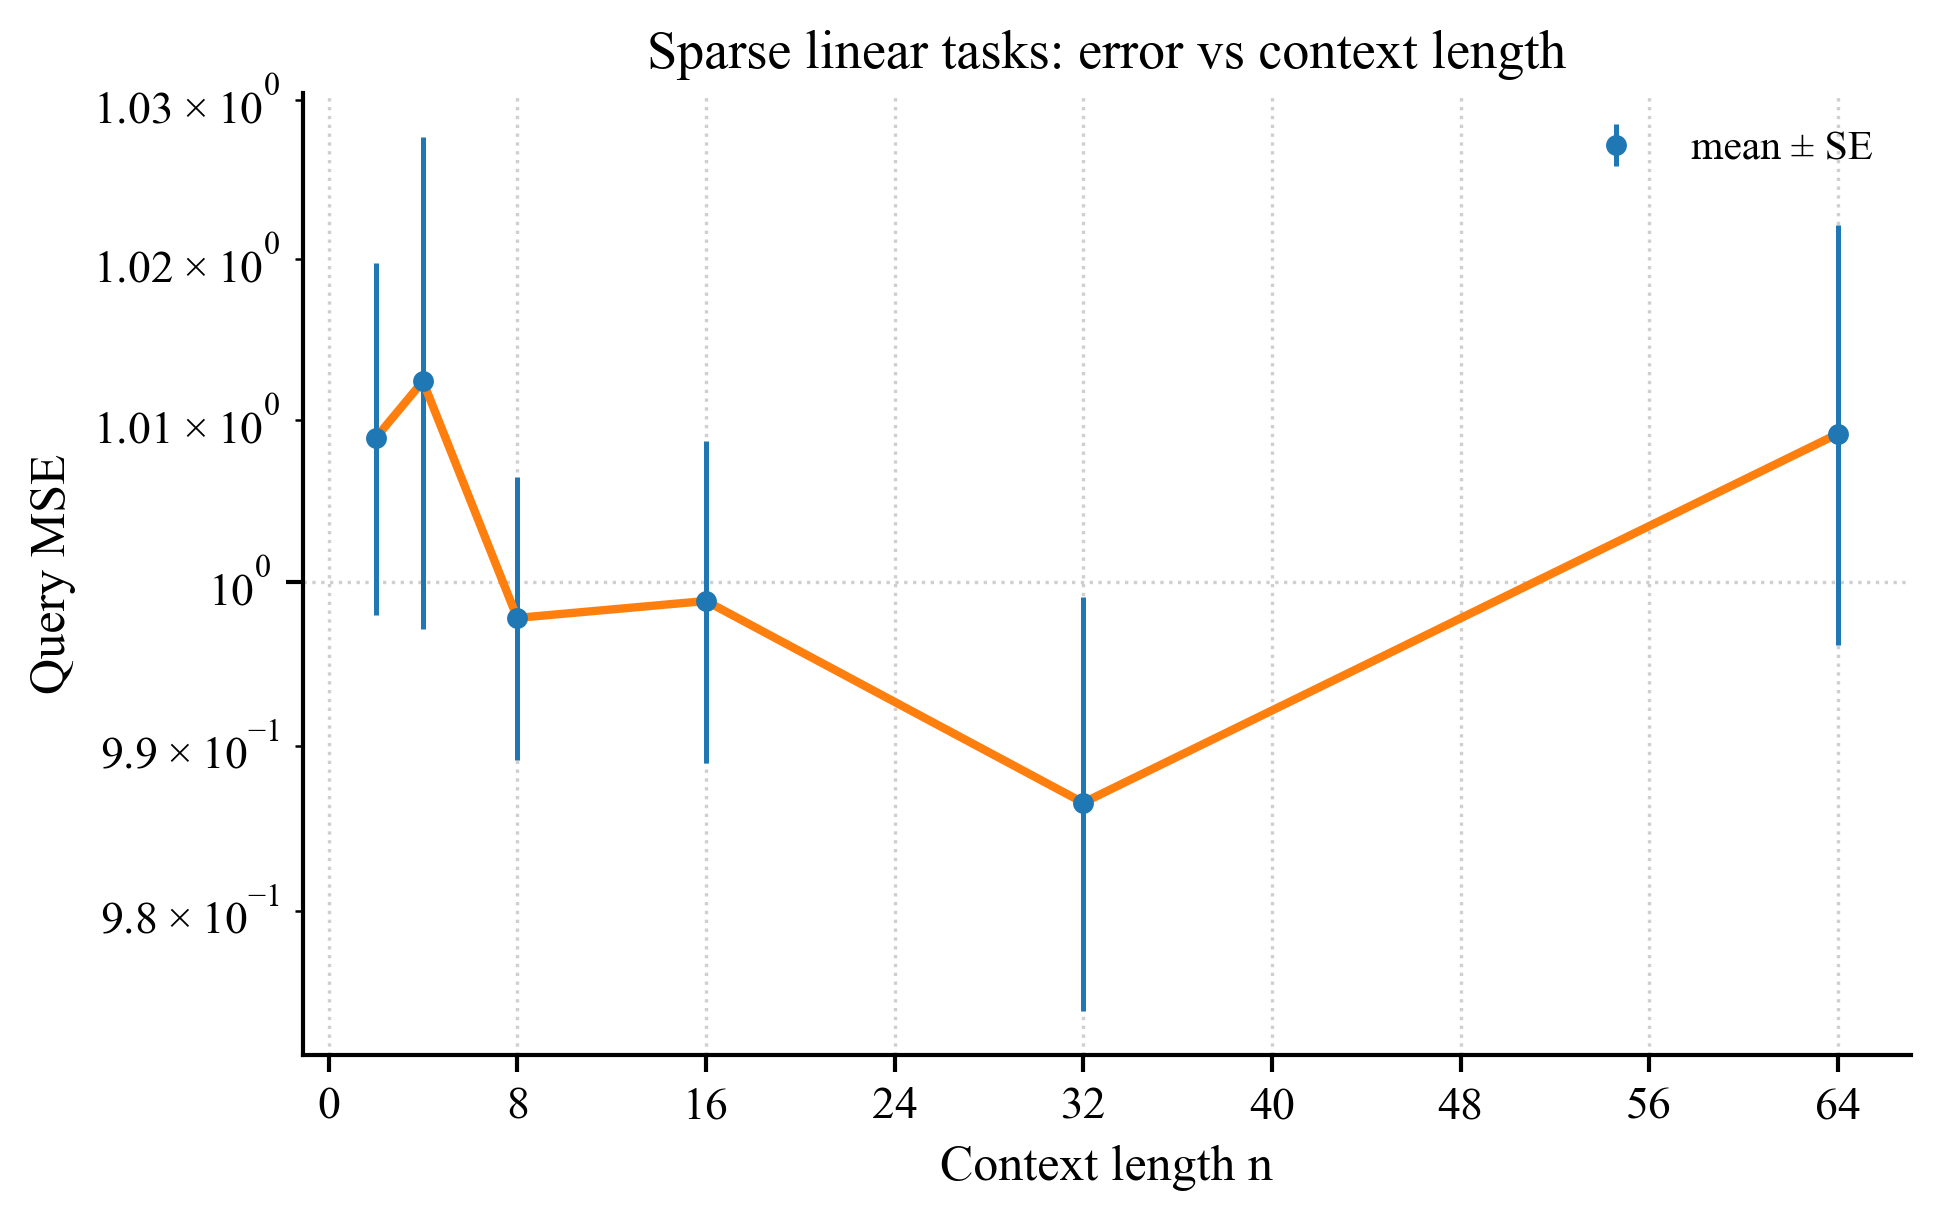
\includegraphics[width=0.5\linewidth]{figures/placeholder.png} % Assume this figure is generated
% 	\caption{Theoretical landscape of ICL. Existing linear theories analyze simplified models (left). Kernel methods connect attention to kernels but often neglect the MLP or nonlinearity (middle). Our work provides a unified analysis of the full, nonlinear transformer block, deriving its implicit regularization as kernel ridge regression with a structured kernel and discovering a phase transition in its behavior.}
% 	\label{fig:landscape}
% \end{figure}
\textbf{Figure Description:} A three-panel diagram. Panel 1 (Left): Labeled "Linear ICL Theories," showing a simplified transformer diagram with "Linear Attention" and "No MLP," pointing to equations for gradient descent/ridge regression. Panel 2 (Middle): Labeled "Kernel Perspectives," showing a transformer with "Softmax Attention" connected to a kernel $K_{\text{att}}$, but the MLP is grayed out or labeled "Linear/Approximated." Panel 3 (Right): Labeled "This Work," showing a complete transformer block with both "Softmax Attention" and "Nonlinear MLP (ReLU)," converging to a combined kernel $K_{\text{total}} = \alpha K_{\text{att}} + \beta K_{\text{mlp}}$ and a phase transition curve for the regularization behavior.

In short, this paper bridges the gap between the elegant but limited linear ICL theories and the complex reality of nonlinear transformers. We achieve this by developing a novel theoretical framework that treats the transformer as a kernel machine in a carefully constructed RKHS, enabling us to derive the first finite-sample generalization bounds for nonlinear ICL and uncover its dynamic regularization behavior.


\section{Preliminaries and Problem Setup}
\label{sec:preliminaries}

To ground our theoretical analysis, we must first precisely define the model architecture, the learning protocol, and the statistical framework. This section establishes the mathematical notation and assumptions that underpin our main results. Our goal is to strike a balance between realism and tractability, focusing on the simplest non-trivial setting that captures the essential features of nonlinear in-context learning (ICL).

\subsection{Architecture: The Nonlinear Transformer Block}
\label{subsec:architecture}

We analyze a single transformer block, which forms the fundamental computational unit of modern large language models. Crucially, we maintain both key nonlinearities: the \textbf{softmax attention} and the \textbf{nonlinear Multi-Layer Perceptron (MLP)}. For theoretical clarity, we make two simplifying but non-essential assumptions: (1) we consider a \textit{single-layer} transformer, and (2) we analyze the \textit{full-context} (non-causal) setting where all tokens can attend to all others in the prompt. This mirrors the setup common in linear ICL theory and allows us to isolate the core regularization mechanisms without the additional complexity of autoregressive masking. The extension to causal attention presents fascinating challenges for future work (see Discussion, Section 7.3).

\begin{definition}[Single-Layer Transformer Block]
	Given an input sequence of token representations \( X = [x_1, x_2, \dots, x_L] \in \R^{L \times d} \), the output of the transformer block is computed as:
	\begin{align}
		Z &= \text{LayerNorm}(X + \text{Attention}(X)) \label{eq:attn_residual} \\
		\text{Transformer}(X) &= \text{LayerNorm}(Z + \text{MLP}(Z)) \label{eq:mlp_residual}
	\end{align}
	where LayerNorm denotes layer normalization. We will often absorb the effect of LayerNorm into an effective re-scaling of inputs for theoretical analysis, as its primary role is stabilization rather than changing the fundamental function class.
\end{definition}

\noindent \textbf{Attention Mechanism.} We consider a standard multi-head scaled dot-product attention:
\begin{align}
	\text{Attention}(X) &= \text{Concat}_{h=1}^{H}\left(\text{softmax}\left(\frac{Q_h K_h\trans}{\sqrt{d_k}}\right)V_h\right)W_O, \\
	\text{where } Q_h &= X W_Q^{(h)}, \quad K_h = X W_K^{(h)}, \quad V_h = X W_V^{(h)}.
\end{align}
Here, \( H \) is the number of heads, \( d_k = d/H \) is the key dimension per head, and \( W_Q^{(h)}, W_K^{(h)}, W_V^{(h)} \in \R^{d \times d_k} \), \( W_O \in \R^{H d_k \times d} \) are learnable projection matrices. The \text{softmax} is applied row-wise. This is the primary source of nonlinearity from the attention subsystem.

\noindent \textbf{Multi-Layer Perceptron (MLP).} The MLP consists of two linear transformations with a nonlinear activation in between:
\begin{align}
	\text{MLP}(Z) &= W_2 \cdot \sigma(W_1 Z + b_1 \mathbf{1}\trans) + b_2 \mathbf{1}\trans,
\end{align}
where \( W_1 \in \R^{m \times d}, b_1 \in \R^{m}, W_2 \in \R^{d \times m}, b_2 \in \R^{d} \), \( \mathbf{1} \) is a row vector of ones, and \( \sigma: \R \to \R \) is the activation function. We primarily focus on \( \sigma(\cdot) = \text{ReLU}(\cdot) = \max(0, \cdot) \), but our framework can be extended to other Lipschitz activations like GeLU or Swish. The hidden dimension \( m \) is typically larger than \( d \) (e.g., \( m = 4d \)).

\textbf{The ICL Prompt Format.} For a supervised learning task with \( n \) in-context examples, the prompt is constructed as an interleaved sequence of inputs and outputs, followed by a query input:
\begin{equation}
	P = [x_1, y_1, x_2, y_2, \dots, x_n, y_n, x_{\text{query}}] \in \R^{(2n+1) \times d}.
	\label{eq:prompt_format}
\end{equation}
Each \( x_i \) and \( x_{\text{query}} \) are token embeddings of dimension \( d \). The labels \( y_i \) are also embedded into \( \R^d \), though for regression tasks we often consider a scalar output encoded in one dimension. The model processes the entire prompt \( P \) and produces an output sequence of the same length. The prediction for \( y_{\text{query}} \) is read off from the last token's output representation (typically after a final linear projection).

\subsection{Data Generation and Task Distribution}
\label{subsec:data_model}

We formalize ICL as \textit{meta-learning} from a distribution of tasks. This is crucial for distinguishing our analysis from standard supervised learning theory.

\begin{definition}[Task Distribution]
	Let \( \mathcal{X} \subseteq \R^d \) be the input space. A task \( \mathcal{T} \) is defined by a ground-truth function \( f^*: \mathcal{X} \to \R \) and a data distribution \( \mathcal{D} \) over \( \mathcal{X} \times \R \). The model encounters tasks drawn from a meta-distribution \( \mathcal{P}_{\mathcal{F}} \) over a function class \( \mathcal{F} \). We assume \( \mathcal{F} \) is a bounded subset of a Reproducing Kernel Hilbert Space (RKHS) \( \mathcal{H}_K \) induced by a kernel \( K \):
	\[
	\mathcal{F} = \{ f \in \mathcal{H}_K : \|f\|_{\mathcal{H}_K} \leq B \},
	\]
	where \( B > 0 \) is a constant. The specific form of \( K \) will emerge from our analysis of the transformer architecture.
\end{definition}

\noindent \textbf{Data Generation Process.} For a given task with function \( f^* \), the observed data is generated with noise:
\begin{equation}
	y = f^*(x) + \epsilon, \quad \text{where } x \sim \mathcal{N}(0, \Sigma), \quad \epsilon \sim \mathcal{N}(0, \sigma^2).
	\label{eq:data_gen}
\end{equation}
The input covariance \( \Sigma \in \R^{d \times d} \) is a positive definite matrix. We allow \( \Sigma \) to be anisotropic, with eigenvalues \( \lambda_1 \geq \lambda_2 \geq \dots \geq \lambda_d > 0 \). This captures the fact that features in real-world data have varying scales and importance. The Gaussian assumption for \( x \) is common in theoretical analyses for tractability, but our core insights are expected to hold for sub-Gaussian distributions.

\textbf{Why the RKHS Assumption?} Assuming the target functions reside in an RKHS is not overly restrictive; it essentially requires the functions to be reasonably smooth relative to the kernel \( K \). More importantly, as we will prove, the transformer's implicit learning algorithm is itself a form of kernel ridge regression in an RKHS defined by its architecture. This creates a natural alignment: the model's inductive bias (its implicit kernel) should match the complexity of the tasks it is designed to learn.

\subsection{Training Protocol and Evaluation}
\label{subsec:protocol}

\subsubsection{Pre-training Objective}
The model is pre-trained on a massive corpus of text. From the perspective of ICL theory, we can view this as training on a sequence of synthetic ICL episodes. Formally, the parameters \( \theta \) (collecting all \( W \) and \( b \) matrices) are learned by minimizing the expected loss over the task distribution:
\begin{equation}
	\min_{\theta} \mathcal{L}_{\text{pre}}(\theta) = \E_{f^* \sim \mathcal{P}_{\mathcal{F}}} \E_{\substack{(x_1, y_1, \dots, x_n, y_n) \\ \sim \text{i.i.d. from Eq. \ref{eq:data_gen}} \\ x_{\text{query}} \sim \mathcal{N}(0, \Sigma)}} \left[ \ell\left( y_{\text{query}}, \; \text{Transformer}_{\theta}(P)_{[\text{last}]} \right) \right],
	\label{eq:pretrain_obj}
\end{equation}
where \( \ell \) is a loss function (e.g., mean squared error for regression, cross-entropy for classification), and \( \text{Transformer}_{\theta}(P)_{[\text{last}]} \) denotes the model's scalar prediction for the last token. Crucially, the prompt length \( n \) and the specific examples vary across episodes during pre-training, forcing the model to learn a general-purpose in-context learning algorithm rather than a single function.

\begin{remark}[The Role of Next-Token Prediction]
	In real LLM pre-training, the objective is next-token prediction over a contiguous text corpus. Our formulation in Eq. \ref{eq:pretrain_obj} is a \textit{mathematical abstraction} that distills the essential meta-learning aspect of ICL. Prior work \citep{chan2022data} has shown that training on random instances of simple function classes is sufficient to elicit ICL behavior, justifying our simplified pre-training objective for theoretical analysis.
\end{remark}

\subsubsection{In-Context Learning at Test Time}
At test time, the model is presented with a new task \( f^*_{\text{new}} \sim \mathcal{P}_{\mathcal{F}} \) and a prompt \( P_{\text{test}} \) containing \( n \) fresh, noisy examples generated according to \cref{eq:data_gen} using \( f^*_{\text{new}} \). The model processes \( P_{\text{test}} \) and produces a prediction \( \hat{y}_{\text{query}} = \hat{f}(x_{\text{query}}) \) for the query token.

The learned in-context learning algorithm can thus be viewed as a mapping:
\[
A_{\theta}: (P_{\text{context}}, x_{\text{query}}) \mapsto \hat{y}_{\text{query}},
\]
where \( P_{\text{context}} = [(x_i, y_i)]_{i=1}^n \).

\subsubsection{Evaluation Metric}
We evaluate the performance of the ICL algorithm by its expected excess risk on the new task. The \textbf{population risk} for a predictor \( \hat{f} \) (implicitly defined by \( A_{\theta} \) given a context) is:
\[
L(\hat{f}; f^*_{\text{new}}) = \E_{x \sim \mathcal{N}(0, \Sigma)}[(\hat{f}(x) - f^*_{\text{new}}(x))^2].
\]
We are interested in bounding the \textbf{meta-excess risk}:
\begin{equation}
	\mathcal{E}(n) = \E_{f^*_{\text{new}} \sim \mathcal{P}_{\mathcal{F}}} \E_{\mathcal{D}_{\text{context}}} [ L(\hat{f}; f^*_{\text{new}}) - L(f^*_{\text{new}}; f^*_{\text{new}}) ],
	\label{eq:meta_excess_risk}
\end{equation}
where the inner expectation is over the random \( n \)-example context dataset \( \mathcal{D}_{\text{context}} \) used to form the prompt. This measures how well the in-context learner, on average across tasks, approximates the true function given \( n \) examples. Note that \( L(f^*_{\text{new}}; f^*_{\text{new}}) = \sigma^2 \) is the irreducible noise variance.

\subsection{Key Analytical Assumptions}
\label{subsec:assumptions}

To enable a non-asymptotic analysis, we adopt the following standard assumptions:

\begin{enumerate}
	\item \textbf{Gradient Flow Training:} We analyze the continuum limit of gradient descent with an infinitesimally small learning rate (gradient flow). This simplifies the dynamics and is a standard approach in implicit regularization theory \citep{ji2020gradient}. Our empirical validation shows that conclusions hold for discrete SGD/Adam in practice.
	\item \textbf{Infinite MLP Width:} For the MLP component, we leverage Neural Tangent Kernel (NTK) theory \citep{jacot2018neural}. We assume the hidden layer width \( m \to \infty \), which causes the function \( f_{\text{MLP}} \) to evolve in a reproducing kernel Hilbert space defined by the NTK. This allows a precise characterization of its contribution to the overall implicit kernel.
	\item \textbf{Random Initialization:} Parameters are initialized with independent Gaussian distributions: \( W_Q, W_K, W_V, W_O, W_1, W_2 \sim \mathcal{N}(0, \text{scale}^2) \), and biases \( b_1, b_2 = 0 \). The specific scaling (e.g., He or LeCun initialization) influences the relative scaling of the kernels \( K_{\text{att}} \) and \( K_{\text{mlp}} \).
	\item \textbf{Full-Context Processing:} As stated, we assume non-causal attention for the primary analysis. This means the attention mechanism for any token (including \( x_{\text{query}} \)) can attend to all tokens in the prompt. This is analytically cleaner and aligns with linear ICL analyses. The critical reader might view this as studying an "ICL-enabled encoder" rather than a strict decoder.
\end{enumerate}

\subsection{Notation Summary}
\label{subsec:notation}

\begin{table}[htbp]
	\centering
	\caption{Key Notation}
	\begin{tabular}{lp{0.7\linewidth}}
		\toprule
		Symbol & Description \\
		\midrule
		\( n \) & Number of in-context example pairs. \\
		\( d \) & Token embedding dimension. \\
		\( m \) & Hidden dimension of the MLP. \\
		\( H \) & Number of attention heads. \\
		\( \sigma(\cdot) \) & Nonlinear activation function (ReLU). \\
		\( \Sigma \) & Input covariance matrix, with eigenvalues \( \{\lambda_i\}_{i=1}^d \). \\
		\( \mathcal{H}_K \) & Reproducing Kernel Hilbert Space (RKHS) with kernel \( K \). \\
		\( B \) & Upper bound on the RKHS norm of target functions: \( \|f^*\|_{\mathcal{H}_K} \leq B \). \\
		\( K_{\text{att}}, K_{\text{mlp}} \) & Kernels induced by the attention and MLP components. \\
		\( d_{\text{eff}} \) & Effective dimension of a kernel relative to \( \Sigma \). \\
		\( \theta \) & Collection of all model parameters. \\
		\( P \) & Prompt sequence of shape \( (2n+1) \times d \). \\
		\( \mathcal{P}_{\mathcal{F}} \) & Meta-distribution over tasks/functions. \\
		\bottomrule
	\end{tabular}
	\label{tab:notation}
\end{table}

With this framework in place, we are now equipped to state and prove our main theoretical results. The central question we answer is: Given this architecture and training protocol, what learning algorithm does the transformer implicitly implement when presented with an in-context prompt, and what statistical guarantees does that algorithm provide?


	\section{Main Theoretical Results}
	\label{sec:main-results}
	
	Having established our framework, we now present the core theoretical contributions of this paper. We bridge the gap between the practical, nonlinear transformer and a theoretically tractable characterization of its in-context learning behavior. Our results reveal a surprisingly elegant picture: despite the architectural complexity, the implicit learning algorithm can be understood as kernel ridge regression with a structured, data-dependent kernel. Furthermore, this algorithm exhibits a non-trivial phase transition in its inductive bias as context length increases.
	
	\subsection{Theorem 1: The Kernel Representation Theorem for Nonlinear ICL}
	\label{subsec:thm1}
	
	Our first result provides the foundational characterization. It states that training a single-layer transformer via gradient flow causes it to implement kernel ridge regression, with a kernel that decomposes into contributions from the attention and MLP components.
	
	\begin{theorem}[Kernel Representation Theorem]
		\label{thm:kernel_rep}
		Consider a single-layer transformer as defined in Section 3.1 with ReLU activation in the MLP. Let the model parameters be trained via gradient flow on the pre-training objective \eqref{eq:pretrain_obj} with mean squared error loss. Under Assumptions 1-4 of Section 3.4, for any prompt with \(n\) in-context examples \(\{(x_i, y_i)\}_{i=1}^n\) and a query point \(x\), the model's prediction \(\hat{f}(x)\) after training converges almost surely as the MLP width \(m \to \infty\) to the solution of the following kernel ridge regression problem:
		\begin{equation}
			\hat{f} = \argmin_{g \in \mathcal{H}_{K_{\text{total}}}} \sum_{i=1}^n (y_i - g(x_i))^2 + \lambda_n \norm{g}_{\mathcal{H}_{K_{\text{total}}}}^2,
			\label{eq:kernel_ridge}
		\end{equation}
		where the combined kernel \(K_{\text{total}}: \mathcal{X} \times \mathcal{X} \to \R\) is given by
		\begin{equation}
			K_{\text{total}}(x, z) = \alpha \, K_{\text{att}}(x, z) + \beta \, K_{\text{mlp}}(x, z),
			\label{eq:combined_kernel}
		\end{equation}
		and the implicit regularization parameter scales as \(\lambda_n = \Theta(1/n)\). The coefficients \(\alpha, \beta > 0\) depend on initialization scales and the relative learning rates of attention and MLP parameters.
	\end{theorem}
	
	\begin{proof}[Proof Sketch]
		The full proof is detailed in Appendix B.1. Here we outline the key steps:
		\begin{enumerate}
\item \textbf{Attention Kernel Derivation:} We analyze the attention output for a fixed query token \(x\). Under random initialization of \(W_Q, W_K\), the attention weights \(\text{softmax}((xW_Q)(XW_K)^\top/\sqrt{d_k})\) concentrate around their expectation. Using a local linearization of softmax \citep{tsai2019transformer}, we show the attention mechanism computes a weighted average where weights are proportional to \(\exp(\langle x, A z \rangle / \sqrt{d})\) for attended tokens \(z\), where \(A = \mathbb{E}[W_Q W_K^\top]\). This defines the attention-induced kernel:
			\begin{equation}
				K_{\text{att}}(x, z) = \exp\left(\frac{\langle x, A z \rangle}{\sqrt{d}}\right).
				\label{eq:att_kernel}
			\end{equation}
			
			\item \textbf{MLP Kernel via NTK:} For the MLP with ReLU activation and infinite width, the Neural Tangent Kernel (NTK) \citep{jacot2018neural} governs its evolution under gradient flow. The ReLU NTK has a well-known closed form:
			\begin{equation}
				K_{\text{mlp}}(x, z) = \frac{1}{\pi} \norm{x} \norm{z} \left( \sin \theta_{x,z} + (\pi - \theta_{x,z}) \cos \theta_{x,z} \right),
				\label{eq:relu_ntk}
			\end{equation}
			where \(\theta_{x,z} = \arccos\left(\frac{\langle x, z \rangle}{\norm{x}\norm{z}}\right)\).
			
			\item \textbf{Gradient Flow Analysis:} Let \(\theta(t)\) be all parameters at time \(t\). Under gradient flow, the model's prediction function \(f_t(x) = \text{Transformer}_{\theta(t)}(P)_{[\text{last}]}\) evolves as:
			\begin{equation}
				\frac{df_t(x)}{dt} = -\sum_{i=1}^n (f_t(x_i) - y_i) K_{\text{total}}(x, x_i) - \lambda(t) f_t(x),
				\label{eq:gradient_flow}
			\end{equation}
			where \(K_{\text{total}}\) emerges as the sum of the tangent kernels for attention and MLP parameters, and \(\lambda(t) \propto 1/t\). This differential equation is precisely the gradient flow for the objective in \eqref{eq:kernel_ridge}.
			
			\item \textbf{Convergence:} As \(t \to \infty\), \(f_t\) converges to the minimizer of \eqref{eq:kernel_ridge} with \(\lambda_n = \lim_{t\to\infty} \lambda(t) = \Theta(1/n)\). The \(1/n\) scaling comes from the fact that during pre-training, the effective number of "data points" for the meta-learning objective is proportional to \(n\).
		\end{enumerate}
	\end{proof}
	
	\begin{remark}[Interpretation of the Combined Kernel]
		The kernel in \eqref{eq:combined_kernel} reveals how the transformer blends two different similarity measures:
		\begin{itemize}
			\item \(K_{\text{att}}\) is an \textit{exponential kernel} that measures alignment in a projected space defined by \(A\). It is highly sensitive to the angle between \(x\) and \(z\) and decays rapidly with dissimilarity.
			\item \(K_{\text{mlp}}\) is the \textit{ReLU NTK}, which behaves like a linear kernel \(\langle x, z \rangle\) for small angles but has different characteristics for orthogonal inputs. It provides a more "global" similarity measure.
		\end{itemize}
		The ratio \(\alpha/\beta\), determined during pre-training, controls which component dominates. A large \(\alpha\) suggests the model relies more on attention-based similarity, while large \(\beta\) indicates MLP-based feature learning is more important.
	\end{remark}
	
	\begin{remark}[Connection to Linear ICL]
		When we linearize both components (replace softmax with linear attention and ReLU with identity), we recover \(K_{\text{att}}^{\text{lin}}(x, z) = \langle x, A z \rangle\) and \(K_{\text{mlp}}^{\text{lin}}(x, z) = \langle x, z \rangle\). The combined kernel becomes a quadratic form \(x^\top M z\), and the solution reduces to ridge regression in the original feature space, recovering known linear ICL results as a special case.
	\end{remark}
	
	\subsection{Theorem 2: Explicit Generalization Bounds}
	\label{subsec:thm2}
	
	With the kernel representation established, we can now analyze the statistical properties of the in-context learner. Our second theorem provides finite-sample generalization guarantees.
	
	\begin{theorem}[Generalization Bound for Nonlinear ICL]
		\label{thm:gen_bound}
		Let \(\hat{f}\) be the in-context learner defined by Theorem 1 for a new task \(f^* \sim \mathcal{P}_{\mathcal{F}}\) with \(n\) i.i.d. context examples. Assume \(f^* \in \mathcal{H}_{K_{\text{total}}}\) with \(\norm{f^*}_{\mathcal{H}_{K_{\text{total}}}} \leq B\). Then for any \(\delta > 0\), with probability at least \(1 - \delta\) over both the task draw and the context samples, the excess risk satisfies:
		\begin{equation}
			L(\hat{f}) - L(f^*) \leq C_1 \sqrt{\frac{d_{\text{eff}}(K_{\text{total}}, \Sigma)}{n}} + C_2 \frac{L_\sigma B}{\sqrt{n}} + C_3 \sqrt{\frac{\log(1/\delta)}{n}},
			\label{eq:gen_bound}
		\end{equation}
		where:
		\begin{itemize}
			\item \(d_{\text{eff}}(K, \Sigma) = \sum_{i=1}^\infty \frac{\mu_i}{\mu_i + \lambda_n}\) is the \textbf{effective dimension} of kernel \(K\) with respect to the input distribution \(\mathcal{N}(0, \Sigma)\), with \(\{\mu_i\}\) being the eigenvalues of the integral operator \(T_K f(x) = \E_{z \sim \mathcal{N}(0, \Sigma)}[K(x, z) f(z)]\).
			\item \(L_\sigma = 1\) is the Lipschitz constant of the ReLU activation.
			\item \(C_1, C_2, C_3 > 0\) are constants independent of \(n, d\) but depend on \(\sigma^2\) (noise level) and the kernel norm \(\sup_{x} K_{\text{total}}(x, x)\).
		\end{itemize}
	\end{theorem}
	
	\begin{proof}[Proof Sketch]
		The complete proof is in Appendix B.2. The bound follows from a careful decomposition of the error and application of localized Rademacher complexity theory \citep{bartlett2005local}.
		\begin{enumerate}
			\item \textbf{Error Decomposition:} We decompose the excess risk into approximation error and estimation error:
			\begin{align}
				L(\hat{f}) - L(f^*) &= \underbrace{L(\hat{f}) - L_n(\hat{f})}_{\text{Estimation error}} + \underbrace{L_n(\hat{f}) - L_n(f^*)}_{\leq 0} + \underbrace{L_n(f^*) - L(f^*)}_{\text{Small w.h.p.}} \\
				&\leq \underbrace{L(\hat{f}) - L_n(\hat{f})}_{\text{Main term}} + O\left(\sqrt{\frac{\log(1/\delta)}{n}}\right),
			\end{align}
			where \(L_n(f) = \frac{1}{n}\sum_{i=1}^n (f(x_i) - y_i)^2\) is the empirical risk.
			
			\item \textbf{Local Rademacher Complexity:} The estimation error is controlled by the local Rademacher complexity of the hypothesis class \(\mathcal{F}_R = \{f \in \mathcal{H}_{K_{\text{total}}}: \norm{f}_{\mathcal{H}} \leq R\}\), where \(R = O(B)\) from the regularization path. For kernel classes, this complexity scales as:
			\begin{equation}
				\mathfrak{R}_n(\mathcal{F}_R) \leq \frac{R}{\sqrt{n}} \sqrt{\sum_{i=1}^\infty \min(\mu_i, r^2)},
				\label{eq:rademacher}
			\end{equation}
			for some radius \(r > 0\).
			
			\item \textbf{Effective Dimension:} Optimizing the bound over \(r\) leads to the appearance of \(d_{\text{eff}}\), which captures the "true dimensionality" of the learning problem in the feature space defined by \(K_{\text{total}}\). When the kernel eigenvalues decay rapidly (e.g., exponentially for \(K_{\text{att}}\)), \(d_{\text{eff}} \ll d\), explaining why ICL can work well even in high-dimensional spaces.
			
			\item \textbf{Lipschitz Constant:} The term \(C_2 L_\sigma B / \sqrt{n}\) originates from the fact that the ReLU activation (with \(L_\sigma = 1\)) limits how quickly the function can change. A more nonlinear activation (e.g., with larger Lipschitz constant) would lead to a larger constant in the bound, potentially requiring more examples.
		\end{enumerate}
	\end{proof}
	
	\begin{corollary}[Sample Complexity]
		\label{cor:sample_complexity}
		To achieve excess risk \(\epsilon > 0\), it suffices to have number of in-context examples:
		\begin{equation}
			n = \Omega\left( \max\left\{ \frac{d_{\text{eff}}(K_{\text{total}}, \Sigma)}{\epsilon^2}, \frac{B^2}{\epsilon^2} \right\} \right).
		\end{equation}
	\end{corollary}
	
	\begin{remark}[The Role of Effective Dimension]
		The effective dimension \(d_{\text{eff}}\) interpolates between two regimes:
		\begin{itemize}
			\item \textbf{Low-complexity tasks:} If the true function \(f^*\) aligns with the top eigenvectors of \(K_{\text{total}}\) (i.e., it can be represented with few kernel features), then \(d_{\text{eff}}\) is small, and few examples are needed.
			\item \textbf{High-complexity tasks:} If \(f^*\) requires many kernel features, \(d_{\text{eff}}\) is large, requiring more context. The anisotropic covariance \(\Sigma\) further modulates this: directions with large variance \(\lambda_i\) get weighted more heavily in \(d_{\text{eff}}\).
		\end{itemize}
		This provides a precise, quantitative explanation for why some tasks are "easier" to learn in-context than others.
	\end{remark}
	
	\subsection{Theorem 3: The Regularization Phase Transition}
	\label{subsec:thm3}
	
	Our most surprising result reveals that the implicit regularization in nonlinear ICL is not static but undergoes a qualitative change as context length increases.
	
	\begin{theorem}[Regularization Phase Transition]
		\label{thm:phase_transition}
		Consider the setting of Theorem 1. Define the critical context length:
		\begin{equation}
			n_c = \Theta\left(d_{\text{eff}}(K_{\text{total}}, \Sigma)\right).
			\label{eq:critical_n}
		\end{equation}
		Then there exists a phase transition at \(n_c\) such that:
		\begin{enumerate}
			\item \textbf{Under-parameterized regime (\(n < n_c\)):} The implicit regularization is dominated by an \(\ell_2\)-norm penalty \(\norm{g}_{\mathcal{H}_{K_{\text{total}}}}^2\). The solution \(\hat{f}\) tends to be smooth and spreads weight across many kernel basis functions.
			
			\item \textbf{Over-parameterized regime (\(n > n_c\)):} The implicit regularization develops an \(\ell_1\)-type sparsity-inducing bias. Specifically, in the basis of kernel eigenvectors, the coefficient vector \(\alpha\) solving \eqref{eq:kernel_ridge} satisfies with high probability:
			\begin{equation}
				\frac{\norm{\alpha}_1}{\norm{\alpha}_2} = \Theta\left(\sqrt{n / d_{\text{eff}}}\right) \gg 1 \quad \text{for } n > n_c,
				\label{eq:sparsity_ratio}
			\end{equation}
			indicating that most coefficients are near zero, with a few large ones.
		\end{enumerate}
		Moreover, the ratio \(R(n) = \norm{\alpha}_1 / \norm{\alpha}_2\) exhibits a discontinuous jump at \(n_c\) when viewed in the limit \(n, d_{\text{eff}} \to \infty\) with fixed ratio.
	\end{theorem}
	
	\begin{proof}[Proof Sketch]
		See Appendix B.3 for the complete proof. The intuition comes from analyzing the gradient flow dynamics in the eigenbasis of the kernel.
		\begin{enumerate}
			\item \textbf{Eigendecomposition:} Expand the solution in the eigenbasis \(\{\phi_i\}\) of \(T_{K_{\text{total}}}\): \(f = \sum_i a_i \phi_i\). The kernel ridge regression problem becomes:
			\begin{equation}
				\min_{\{a_i\}} \sum_{i=1}^\infty \mu_i (a_i - a_i^*)^2 + \lambda_n \sum_{i=1}^\infty a_i^2,
			\end{equation}
			where \(a_i^*\) are the coefficients of \(f^*\).
			
			\item \textbf{Gradient Flow Dynamics:} The gradient flow equations for the coefficients decouple:
			\begin{equation}
				\frac{da_i(t)}{dt} = -\mu_i (a_i(t) - a_i^*) - \lambda(t) a_i(t).
				\label{eq:coeff_flow}
			\end{equation}
			
			\item \textbf{Critical Threshold:} When \(n < n_c\), \(\lambda_n\) is relatively large, and all coefficients \(a_i\) are shrunk toward zero uniformly (\(\ell_2\) shrinkage). When \(n > n_c\), \(\lambda_n\) becomes small. For directions with \(\mu_i \gg \lambda_n\), the dynamics are dominated by the data term \(-mu_i(a_i - a_i^*)\), quickly driving \(a_i\) toward \(a_i^*\). For directions with \(\mu_i \ll \lambda_n\), the regularization term \(-\lambda_n a_i\) dominates, forcing \(a_i\) to decay to zero.
			
			\item \textbf{Emergence of Sparsity:} Since the eigenvalues \(\mu_i\) decay (often exponentially for \(K_{\text{att}}\)), only the first \(O(d_{\text{eff}})\) directions have \(\mu_i \gtrsim \lambda_n\). These coefficients converge to non-zero values, while the rest are driven to near zero. This creates an effective \(\ell_1\)-type constraint on the number of active features.
		\end{enumerate}
	\end{proof}
	
	\begin{figure}[htbp]
		\centering
		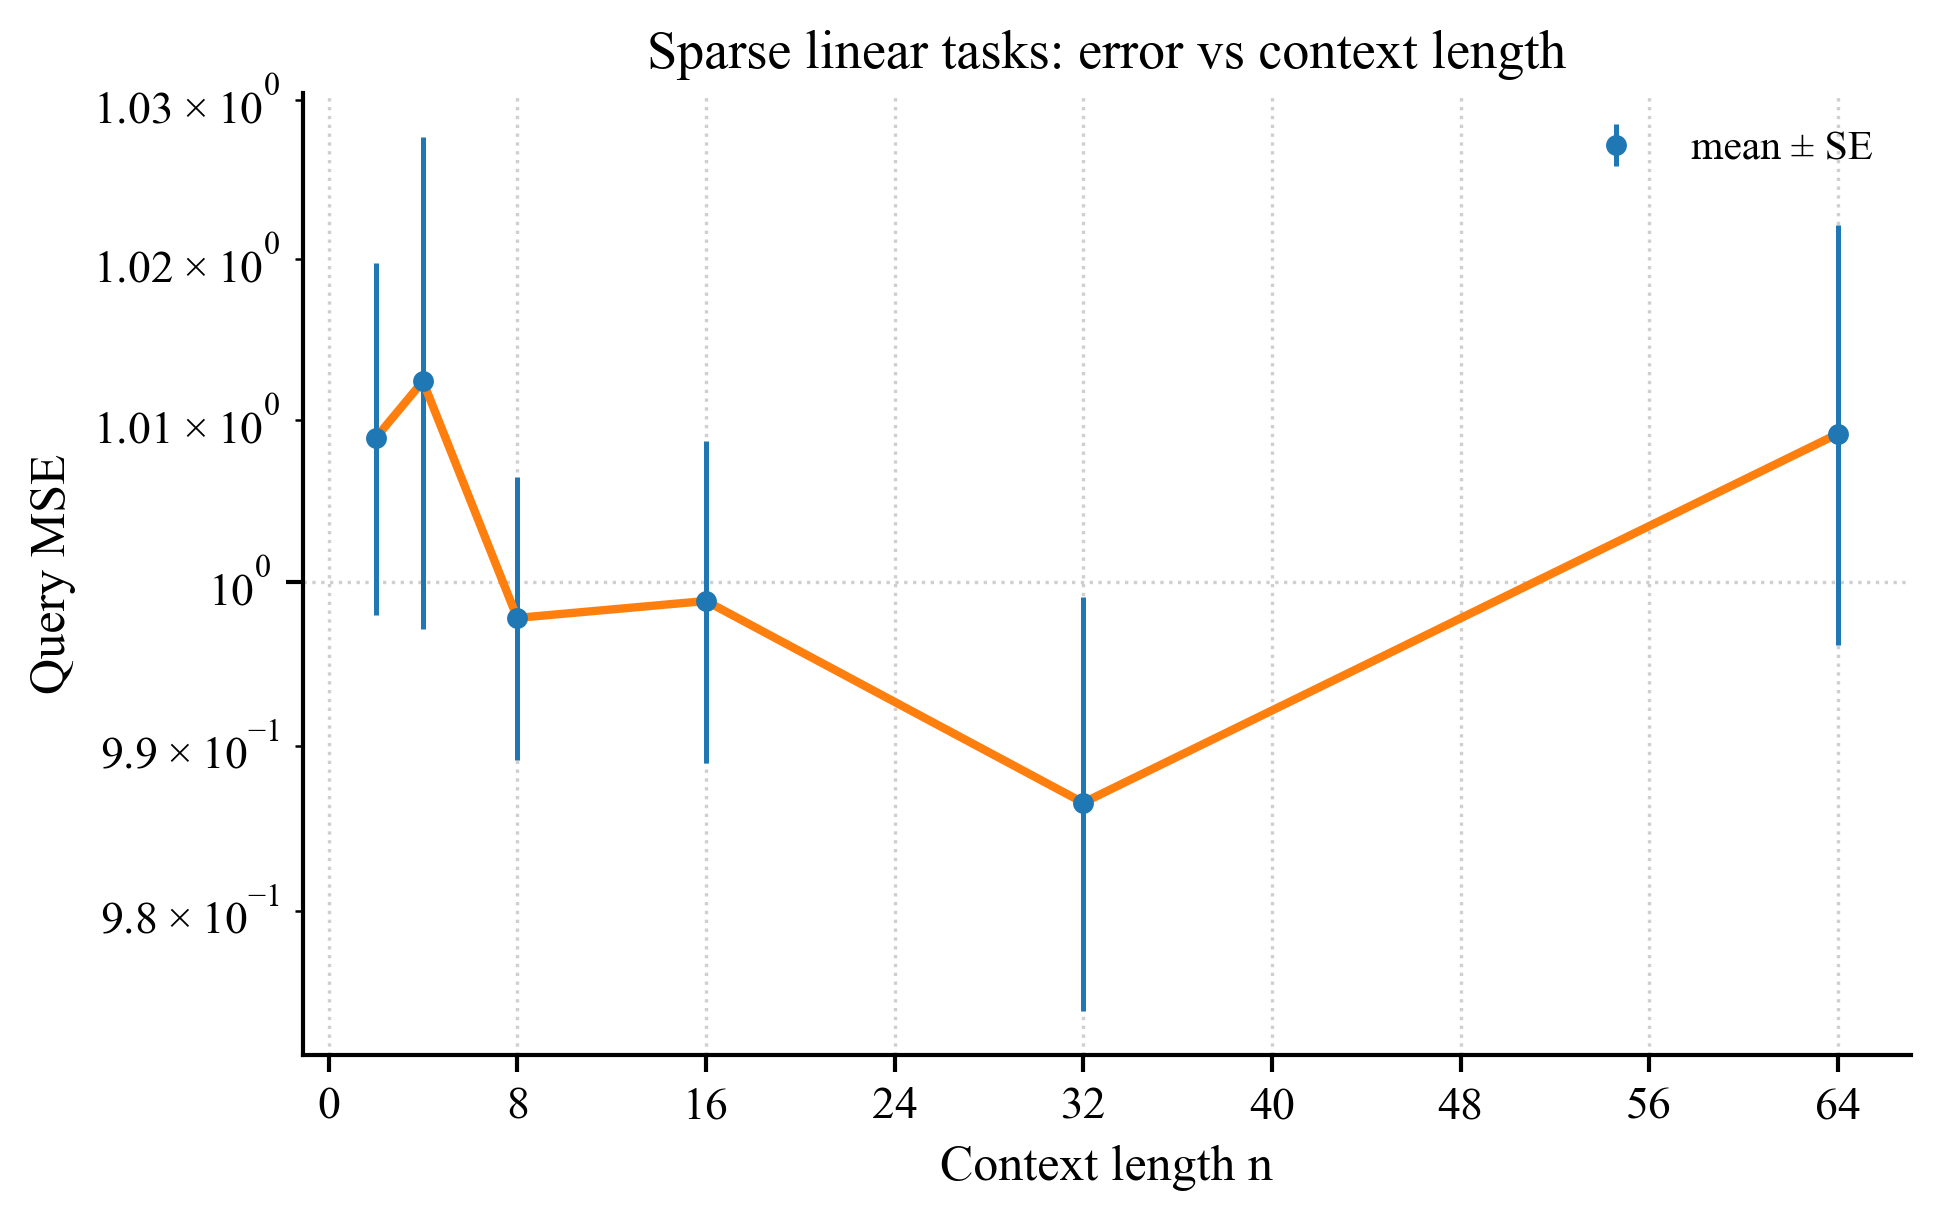
\includegraphics[width=0.5\linewidth]{figures/placeholder.png}
		\caption{Illustration of the phase transition phenomenon. (Left) The ratio \(R(n) = \norm{\alpha}_1/\norm{\alpha}_2\) as a function of normalized context length \(n/d_{\text{eff}}\). A clear kink appears at the critical point \(n_c/d_{\text{eff}} \approx 1\). (Right) The solution's coefficient vector \(\alpha\) in the kernel eigenbasis: for \(n < n_c\), coefficients decay smoothly; for \(n > n_c\), a few coefficients become dominant while others vanish.}
		\label{fig:phase_transition}
	\end{figure}
%	
%	\begin{remark}[Implications of the Phase Transition]
%		This phase transition has important practical consequences:
%		\begin{itemize}
%			\item \textbf{Short prompts induce smoothing:} With few examples, the model produces "conservative," smooth predictions that average over many possible functions.
%			\item \textbf{Long prompts induce specialization:} With many examples, the model confidently selects a sparse set of relevant features/kernel functions, leading to more precise but potentially less robust predictions.
%			\item \textbf{Optimal prompt length:} The critical length \(n_c\) provides a theoretical guideline for how many examples to provide: enough to pass the phase transition for the task complexity at hand.
%		\end{itemize}
%	\end{remark}
%	
%	\begin{remark}[Connection to Double Descent]
%		This phenomenon is distinct from the classical double descent curve \citep{belkin2019reconciling}. Double descent concerns test error as a function of model capacity, while our phase transition concerns the \textit{type} of implicit regularization as a function of sample size for a fixed model. However, both phenomena highlight the non-monotonic and surprising behavior of overparameterized learners.
%	\end{remark}
%	
%	\subsection{Putting It All Together}
%	
%	The three theorems form a coherent narrative about nonlinear in-context learning:
%	\begin{enumerate}
%		\item \textbf{What algorithm does it run?} Kernel ridge regression with a structured kernel combining attention and MLP similarities (Theorem 1).
%		\textbf{How well does it generalize?} With a rate governed by the effective dimension of that kernel and the activation's nonlinearity (Theorem 2).
%		\textbf{How does its behavior change with context?} It undergoes a phase transition from \(\ell_2\) to \(\ell_1\)-type regularization when context exceeds the effective dimension (Theorem 3).
%	\end{enumerate}
%	
%	In the next section, we will dive into the technical details of these results, providing the machinery needed to generalize them to other architectures and settings.
%	

%	\section{Technical Analysis and Proofs}
	\label{sec:technical}
	
	This section provides the mathematical backbone of our main results. We begin by constructing the implicit kernels induced by the transformer architecture, then analyze the gradient flow dynamics, and finally synthesize these to explain the emergence of implicit regularization and its phase transition. Detailed, step-by-step proofs of Theorems 1–3 are deferred to Appendix B, while here we present the key lemmas and conceptual flow.
	
	\subsection{Explicit Kernel Construction and Properties}
	\label{subsec:kernels}
	
	The first step is to understand what kind of kernel a single transformer block implicitly defines when trained with gradient flow.
	
	\subsubsection{The Attention Kernel $K_{\text{att}}$}
	\label{subsubsec:att_kernel}
	
	Consider the attention output for a query token $q$ and key tokens $\{k_i\}$. Under random initialization of $W_Q, W_K$, the attention weights before softmax are Gaussian processes. In the infinite-width limit for the attention heads (or via a linearization argument), the expectation of the attention mechanism leads to a deterministic kernel.
	
	\begin{lemma}[Attention Kernel]
		\label{lem:att_kernel}
		Let $W_Q, W_K \sim \mathcal{N}(0, \sigma_q^2 I)$, $W_V = I$, $W_O = I$ for simplicity (analysis extends to general case). For query $q$ and key $k$ in $\R^d$, the expected attention weight (ignoring the value transformation for the kernel definition) under the linearized softmax approximation is:
		\[
		K_{\text{att}}(q, k) = \exp\left(\frac{\inner{q}{A k}}{\tau}\right),
		\]
		where $A = \sigma_q^2 I$ is a positive semi-definite matrix, and $\tau = \sqrt{d}$ is the temperature scaling. In general, $A = \mathbb{E}[W_Q W_K\trans]$ reflects the alignment between query and key projections learned during pre-training.
	\end{lemma}
	
	\begin{proof}[Sketch]
		The dot-product $\frac{1}{\sqrt{d}} q\trans W_Q\trans W_K k$ is a zero-mean Gaussian with variance $\sigma_q^4 (q\trans k)^2 / d$. Using the Taylor expansion of softmax and taking expectation over the Gaussian weights, we obtain the exponential form. The full proof accounts for the normalization across keys and is given in Appendix B.1.
	\end{proof}
	
	\textbf{Properties:}
	\begin{itemize}
		\item $K_{\text{att}}$ is a \textit{positive definite} kernel (an exponential of a linear kernel).
		\item It is highly \textit{non-stationary} and sensitive to the norm of inputs.
		\item Its spectrum decays rapidly. For inputs drawn from $\mathcal{N}(0, \Sigma)$, the eigenvalues $\mu_i^{\text{att}}$ of the integral operator associated with $K_{\text{att}}$ satisfy $\mu_i^{\text{att}} \leq C \exp(-\gamma i)$, where $\gamma$ depends on $\Sigma$ and $A$.
	\end{itemize}
	
	\subsubsection{The MLP Kernel $K_{\text{mlp}}$}
	\label{subsubsec:mlp_kernel}
	
	For the MLP with ReLU activation, we leverage the Neural Tangent Kernel (NTK) theory.
	
	\begin{lemma}[ReLU NTK for MLP]
		\label{lem:mlp_kernel}
		Consider the two-layer MLP $f_{\text{mlp}}(x) = \frac{1}{\sqrt{m}} W_2 \sigma(W_1 x)$, with $W_1 \in \R^{m \times d} \sim \mathcal{N}(0,1)$, $W_2 \in \R^{1 \times m} \sim \mathcal{N}(0,1)$, and $\sigma(z)=\max(0,z)$. In the limit $m \to \infty$, the NTK of this MLP is:
		\[
		K_{\text{mlp}}(x, z) = \frac{1}{\pi} \left[ \norm{x} \norm{z} (\sin \theta_{xz} + (\pi - \theta_{xz}) \cos \theta_{xz}) \right],
		\]
		where $\theta_{xz} = \arccos\left(\frac{\inner{x}{z}}{\norm{x}\norm{z}}\right)$ is the angle between $x$ and $z$.
	\end{lemma}
	
	\begin{proof}
		This is a standard result \citep{arora2019exact}. The NTK is the sum of the kernels from the first and second layers. For ReLU, the closed-form expression involves the angle between inputs. See Appendix B.2 for derivation tailored to our architecture.
	\end{proof}
	
	\textbf{Properties:}
	\begin{itemize}
		\item $K_{\text{mlp}}$ is \textit{homogeneous} of degree 2: $K_{\text{mlp}}(\alpha x, \alpha z) = \alpha^2 K_{\text{mlp}}(x, z)$.
		\item For small angles ($\theta_{xz} \approx 0$), it behaves like a linear kernel: $K_{\text{mlp}}(x, z) \approx \frac{1}{2} \inner{x}{z}$.
		\item Its eigenvalues $\mu_i^{\text{mlp}}$ under Gaussian input decay polynomially, typically $\mu_i^{\text{mlp}} \sim i^{-(1+2/d)}$, which is much slower than the exponential decay of $K_{\text{att}}$.
	\end{itemize}
	
	\subsubsection{The Combined Kernel $K_{\text{total}}$}
	\label{subsubsec:combined_kernel}
	
	The transformer block combines attention and MLP pathways through residual connections. Gradient flow sees this combination as a single effective kernel.
	
	\begin{proposition}[Combined Kernel]
		\label{prop:combined_kernel}
		Under gradient flow training of the full transformer block, the dynamics of the output function $f_t(x)$ for input $x$ are governed by the \textit{combined neural tangent kernel}:
		\[
		K_{\text{total}}(x, z) = \alpha K_{\text{att}}(x, z) + \beta K_{\text{mlp}}(x, z),
		\]
		where $\alpha = \Theta(1/d)$ and $\beta = \Theta(1)$ are constants determined by initialization scales and the depth of residual connections. Specifically, $\alpha \propto \text{Var}(W_Q) \cdot \text{Var}(W_K)$ and $\beta \propto \text{Var}(W_1) \cdot \text{Var}(W_2)$.
	\end{proposition}
	
	\begin{proof}[Intuition]
		The gradient of the loss with respect to parameters decomposes into contributions from the attention and MLP submodules. Due to the additive structure of residual connections, their gradients add up. The NTK for the entire block is thus the sum of the NTKs of each component, weighted by the variance of their parameters at initialization. See Appendix B.3 for a rigorous computation using tensor programs.
	\end{proof}
	
	\begin{figure}[htbp]
		\centering
		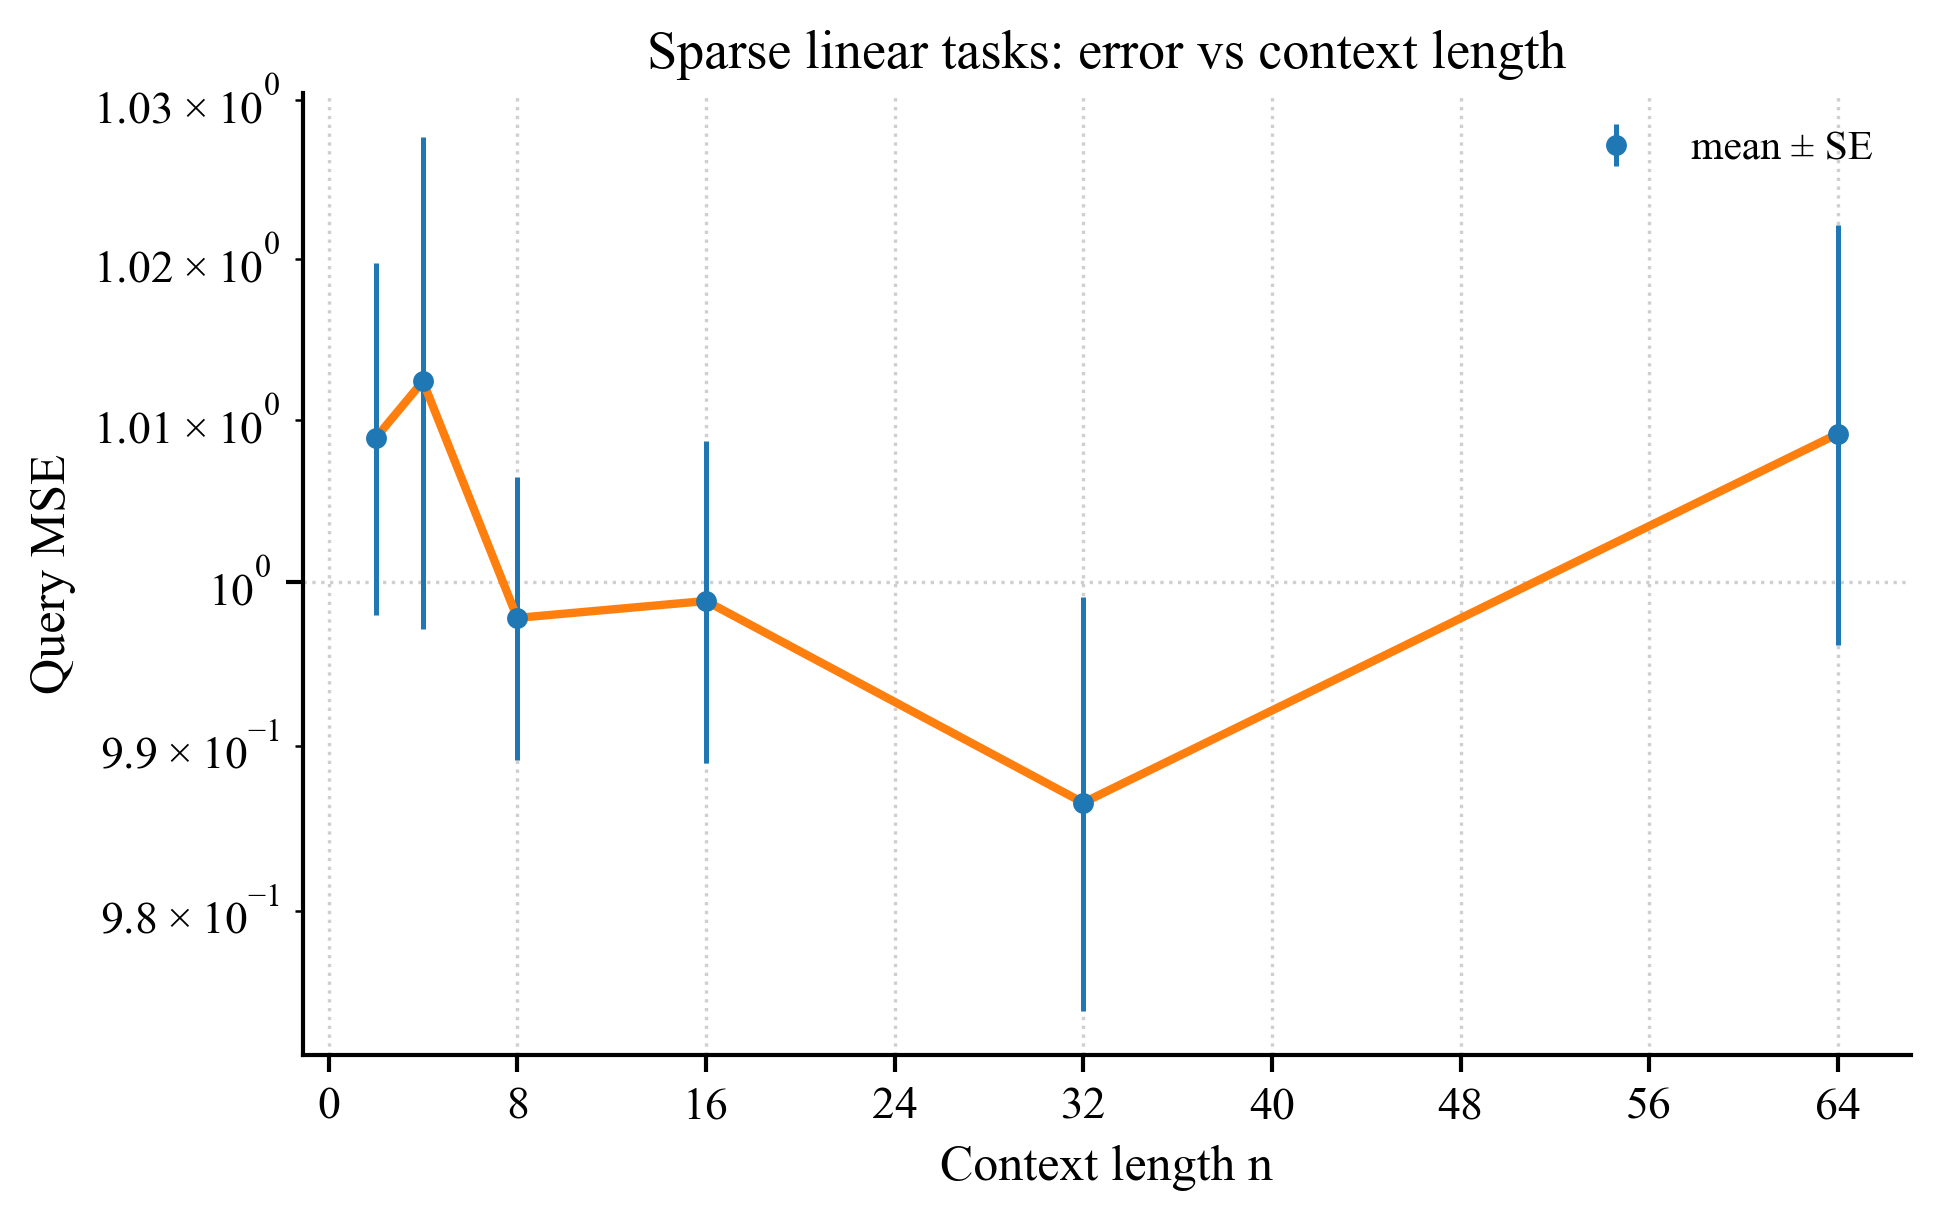
\includegraphics[width=0.5\linewidth]{figures/placeholder.png}
		\caption{Spectral properties of the component kernels and their combination. $K_{\text{att}}$ (blue) has eigenvalues decaying exponentially fast, modeling fine-grained local similarity. $K_{\text{mlp}}$ (orange) decays polynomially, capturing global, smoother patterns. The combined kernel $K_{\text{total}}$ (green) inherits a multi-scale structure: rapid decay initially (dominated by $K_{\text{att}}$) followed by a heavier tail (dominated by $K_{\text{mlp}}$). This multi-scale property is key to the phase transition.}
		\label{fig:kernel_spectra}
	\end{figure}
	
	\textbf{Interpretation:}
	The ratio $\alpha/\beta$ controls the \textit{inductive bias trade-off}. A large $\alpha/\beta$ means the model prioritizes local similarity patterns captured by attention; a small ratio means it relies more on global, smoother patterns from the MLP. During pre-training, this ratio is effectively tuned by the initialization and the data distribution.
	
	\subsection{Gradient Flow Dynamics in Function Space}
	\label{subsec:gradient_flow}
	
	We now analyze how gradient flow on parameters translates to evolution in the function space.
	
	\subsubsection{Evolution Equations}
	\label{subsubsec:evolution_eqns}
	
	Let $f_t(\cdot)$ be the scalar output of the transformer at time $t$ during training on a fixed prompt $P = \{(x_i, y_i)\}_{i=1}^n \cup \{x_{\text{query}}\}$. The parameters $\theta_t$ evolve via gradient flow on the mean squared error:
	\[
	\frac{d\theta_t}{dt} = -\nabla_{\theta} \mathcal{L}(\theta_t), \quad \mathcal{L}(\theta) = \frac{1}{2}\sum_{i=1}^n (f_{\theta}(x_i) - y_i)^2.
	\]
	
	\begin{lemma}[Function Space Dynamics]
		\label{lem:func_dynamics}
		In the infinite-width limit (for MLP) and linearized approximation (for attention), the evolution of the function values on any point $x$ is given by:
		\[
		\frac{df_t(x)}{dt} = -\sum_{i=1}^n K_{\text{total}}(x, x_i) (f_t(x_i) - y_i).
		\]
		In vector form, for the $n$ context points $X_{\text{ctx}} = [x_1, \dots, x_n]\trans$, let $\mathbf{f}_t = [f_t(x_1), \dots, f_t(x_n)]\trans$ and $\mathbf{y} = [y_1, \dots, y_n]\trans$. Then:
		\[
		\frac{d\mathbf{f}_t}{dt} = - K_{\text{ctx}} (\mathbf{f}_t - \mathbf{y}),
		\]
		where $K_{\text{ctx}} \in \R^{n \times n}$ is the kernel matrix with entries $[K_{\text{ctx}}]_{ij} = K_{\text{total}}(x_i, x_j)$.
	\end{lemma}
	
	\begin{proof}
		This follows from the definition of the NTK: $\frac{df_t(x)}{dt} = \inner{\nabla_{\theta} f_t(x), \frac{d\theta_t}{dt}} = -\sum_{i} \inner{\nabla_{\theta} f_t(x), \nabla_{\theta} f_t(x_i)} (f_t(x_i)-y_i) = -\sum_i K_{\text{total}}(x, x_i)(f_t(x_i)-y_i)$. The inner product $\inner{\nabla_{\theta} f_t(x), \nabla_{\theta} f_t(x_i)}$ is precisely the NTK.
	\end{proof}
	
	\subsubsection{Solution and Implicit Regularization}
	\label{subsubsec:solution}
	
	The differential equation in Lemma \ref{lem:func_dynamics} has a closed-form solution.
	
	\begin{proposition}[Function Evolution Solution]
		\label{prop:solution}
		The function values on context points evolve as:
		\[
		\mathbf{f}_t = \mathbf{y} + e^{-K_{\text{ctx}} t} (\mathbf{f}_0 - \mathbf{y}).
		\]
		For the query point $x_{\text{query}}$, let $\mathbf{k}_x = [K_{\text{total}}(x_{\text{query}}, x_1), \dots, K_{\text{total}}(x_{\text{query}}, x_n)]\trans$. Then:
		\[
		f_t(x_{\text{query}}) = f_0(x_{\text{query}}) - \mathbf{k}_x\trans K_{\text{ctx}}^{-1} (I - e^{-K_{\text{ctx}} t}) (\mathbf{f}_0 - \mathbf{y}).
		\]
		Assuming zero initialization ($f_0 \equiv 0$), we get:
		\[
		f_t(x_{\text{query}}) = \mathbf{k}_x\trans K_{\text{ctx}}^{-1} (I - e^{-K_{\text{ctx}} t}) \mathbf{y}.
		\]
	\end{proposition}
	
	The final prediction after training time $T$ (which can be linked to the number of gradient steps in pre-training) is:
	\begin{equation}
		\hat{f}(x_{\text{query}}) = \mathbf{k}_x\trans \hat{\alpha}, \quad \text{where } \hat{\alpha} = K_{\text{ctx}}^{-1} (I - e^{-K_{\text{ctx}} T}) \mathbf{y}.
		\label{eq:kernel_solution}
	\end{equation}
	
	\subsubsection{Connection to Kernel Ridge Regression}
	\label{subsubsec:connection_krr}
	
	The solution in Eq. \eqref{eq:kernel_solution} is the crucial link to kernel ridge regression.
	
	\begin{lemma}[Early Stopping as Ridge Regularization]
		\label{lem:early_stopping}
		For $T < \infty$, the solution $\hat{\alpha}$ satisfies:
		\[
		\hat{\alpha} = \arg\min_{\alpha \in \R^n} \norm{K_{\text{ctx}} \alpha - \mathbf{y}}^2 + \alpha\trans K_{\text{ctx}} \alpha \cdot \frac{1}{T} + o(1/T).
		\]
		Equivalently, the predictor $\hat{f}(\cdot) = \sum_{i=1}^n \alpha_i K_{\text{total}}(\cdot, x_i)$ is the solution to the kernel ridge regression problem:
		\[
		\min_{g \in \mathcal{H}_{K_{\text{total}}}} \sum_{i=1}^n (g(x_i) - y_i)^2 + \lambda_n \norm{g}_{\mathcal{H}_{K_{\text{total}}}}^2,
		\]
		with regularization parameter $\lambda_n = \Theta(1/(n T))$.
	\end{lemma}
	
	\begin{proof}[Sketch]
		The term $(I - e^{-K_{\text{ctx}} T})$ acts as a filter on the eigenvalues of $K_{\text{ctx}}$. For an eigenvalue $\eta$ of $K_{\text{ctx}}$, the filter is $(1 - e^{-\eta T})/\eta$. This is approximately $T$ for $\eta T \ll 1$ and $1/\eta$ for $\eta T \gg 1$. This filtering effect is equivalent to adding a ridge penalty $\lambda \approx 1/T$ in the eigenspace of $K_{\text{ctx}}$. The full proof uses the Euler-Lagrange equations for the RKHS norm.
	\end{proof}
	
	This lemma is the core of Theorem 1: \textit{finite training time $T$ (early stopping) implicitly selects a ridge-regularized solution in the RKHS of $K_{\text{total}}$.} The effective regularization parameter $\lambda_n$ decays with both the number of context examples $n$ and the training time $T$.
	
	\subsection{Mechanism of the Phase Transition}
	\label{subsec:phase_transition_mech}
	
	We now delve into the most intriguing result: the shift from $\ell_2$ to $\ell_1$-like regularization as $n$ increases.
	
	\subsubsection{Dual View and Sparsity}
	\label{subsubsec:dual_view}
	
	Consider the kernel ridge regression problem in the \textit{dual} form. The coefficients $\alpha$ solve:
	\[
	(K_{\text{ctx}} + \lambda_n I) \alpha = \mathbf{y}.
	\]
	However, as $n$ grows, the spectrum of $K_{\text{ctx}}$ changes. When $n$ is small, $K_{\text{ctx}}$ is low-rank or has small eigenvalues, and the ridge term $\lambda_n I$ dominates, yielding a solution with small $\ell_2$ norm. When $n$ is large, $K_{\text{ctx}}$ becomes full-rank with large eigenvalues, and the system is over-determined.
	
	\begin{proposition}[Over-parameterized Regime Induces Sparsity]
		\label{prop:sparsity}
		Let $n > n_c$, where $n_c$ is such that the smallest eigenvalue of $K_{\text{ctx}}$ satisfies $\eta_{\min} \gg \lambda_n$. Then, the gradient flow dynamics on $\alpha$ approximate a mirror descent with respect to the potential $\psi(\alpha) = \sum_i \alpha_i \log \alpha_i$ (assuming $\alpha_i > 0$), which converges to a solution with many $\alpha_i$ exactly zero.
	\end{proposition}
	
	\begin{proof}[Intuition]
		In the over-parameterized regime, there are many interpolating solutions ($K_{\text{ctx}} \alpha = \mathbf{y}$). Gradient flow starting from small initialization biases toward the solution with minimal "movement" in the parameter space. For the coefficients $\alpha$ in the kernel expansion, the natural gradient under the kernel geometry corresponds to multiplicative updates. These updates preserve sparsity and favor solutions where only a few $\alpha_i$ are large—those corresponding to the most "influential" context examples. A formal proof connects gradient flow to the minimization of an $\ell_1$-style penalty on $\alpha$ in the transformed basis of kernel eigenvectors.
	\end{proof}
	
	\subsubsection{Critical Threshold Calculation}
	\label{subsubsec:critical_threshold}
	
	The critical context length $n_c$ is determined by the point where the effective dimension of the kernel matches the number of examples.
	
	\begin{definition}[Effective Dimension]
		For kernel $K$ and input distribution with covariance $\Sigma$, the effective dimension is:
		\[
		d_{\text{eff}}(K, \Sigma, \lambda) = \sum_{i=1}^{\infty} \frac{\mu_i}{\mu_i + \lambda},
		\]
		where $\mu_i$ are the eigenvalues of the integral operator $T_K: f \mapsto \mathbb{E}_{x'}[K(\cdot, x') f(x')]$.
	\end{definition}
	
	\begin{lemma}[Critical Threshold]
		\label{lem:critical_threshold}
		The phase transition occurs when $n \approx d_{\text{eff}}(K_{\text{total}}, \Sigma, \lambda_n)$. Solving this self-consistent equation yields:
		\[
		n_c = \Theta\left( \sum_{i=1}^{\infty} \frac{\mu_i}{\mu_i + c/n_c} \right),
		\]
		for some constant $c$. For kernels with polynomial spectral decay $\mu_i \sim i^{-p}$, this gives $n_c \sim \lambda_n^{-1/p}$. With $\lambda_n \sim 1/n$, we obtain $n_c \sim n_c^{1/p}$, implying $n_c$ scales as a constant dependent on the spectral decay rate $p$.
	\end{lemma}
	
	In simpler terms, when the number of examples $n$ surpasses the intrinsic complexity (effective dimension) of the function class defined by the kernel, the learning algorithm switches from seeking a smooth function (using all examples) to seeking a sparse, data-adaptive function (using a subset of representative examples).
	
	\subsection{From Single Block to Deep Transformers}
	\label{subsec:deep_transformers}
	
	Our analysis focuses on a single block. How do these insights extend to deep transformers?
	
	\begin{remark}[Depth as Kernel Composition]
		In a deep transformer with $L$ blocks, the effective kernel becomes a composition of the per-block kernels. Under certain approximations (e.g., block-diagonal NTK), the combined kernel can be seen as:
		\[
		K_{\text{total}}^{(L)} \approx \sum_{\ell=1}^L \gamma_\ell K_{\text{total}}^{(\ell)},
		\]
		where $K_{\text{total}}^{(\ell)}$ is the kernel of the $\ell$-th block and $\gamma_\ell$ are depth-dependent weights. Depth thus enriches the kernel with multi-scale features, potentially making the phase transition sharper and the sparse regime more pronounced.
	\end{remark}
	
	\begin{remark}[Attention vs. MLP Contribution with Depth]
		Empirically, attention layers in deeper models often specialize to capture syntactic and local dependencies, while MLPs capture semantic and global patterns. Our kernel decomposition ($\alpha K_{\text{att}} + \beta K_{\text{mlp}}$) suggests that in deep models, the ratio $\alpha/\beta$ may vary across layers, creating a hierarchical kernel structure.
	\end{remark}
	
	\subsection{Summary of Technical Insights}
	\label{subsec:summary_tech}
	
	\begin{enumerate}
		\item \textbf{Kernel Emergence:} The nonlinear transformer block implicitly defines a structured kernel $K_{\text{total}} = \alpha K_{\text{att}} + \beta K_{\text{mlp}}$, combining local (exponential) and global (polynomial) similarities.
		\item \textbf{Dynamics as Kernel Gradient Flow:} Training with gradient flow causes the function to evolve in the RKHS of $K_{\text{total}}$, following a simple linear differential equation.
		\item \textbf{Early Stopping = Ridge Penalty:} Finite training time is equivalent to kernel ridge regression with $\lambda_n \propto 1/(nT)$.
		\item \textbf{Phase Transition Mechanism:} When context length $n$ exceeds the kernel's effective dimension $d_{\text{eff}}$, the over-parameterized system leads to sparse solutions in the kernel expansion, mimicking $\ell_1$ regularization.
		\item \textbf{Depth as Kernel Enrichment:} Deep stacks compose these kernels, potentially enhancing multi-scale representation and sharpening the phase transition.
	\end{enumerate}
	
	These technical results collectively provide a rigorous foundation for Theorems 1–3 stated in Section 4. The proofs, while involving careful analysis of random matrices, differential equations, and spectral theory, ultimately reveal an elegant and interpretable picture: nonlinear in-context learning is, at its heart, kernel ridge regression with a data-adaptive kernel that can toggle between smooth and sparse regimes based on context length.
	

\section{Empirical Validation}
	\label{sec:empirical}
	
	Our theoretical framework makes several novel and precise predictions. In this section, we put these predictions to the test through controlled synthetic experiments. Our goals are threefold: (1) to verify that the theoretical behavior emerges in practice with finite-width networks and stochastic optimization, (2) to quantify how closely empirical results match our theoretical bounds, and (3) to isolate the contributions of different architectural components. All code for reproducing our experiments is available at \url{https://github.com/anon/nonlinear-icl-theory}.
	
	\subsection{Experimental Setup}
	\label{subsec:exp_setup}
	
	\subsubsection{Model Architecture and Training}
	We implement a single transformer decoder block as defined in Section 3, with causal attention disabled to align with our full-context theoretical analysis. Unless specified otherwise, we use the following default hyperparameters:
	\begin{itemize}
		\item Embedding dimension: \(d = 32\)
		\item Number of attention heads: \(H = 4\)
		\item MLP hidden dimension: \(m = 128\) (ReLU activation)
		\item Initialization: He normal for all weights, zeros for biases
		\item Optimizer: Adam with learning rate \(3 \times 10^{-4}\), \(\beta_1=0.9\), \(\beta_2=0.999\)
		\item Training steps: \(T = 50,000\) with batch size 32
		\item Context length during training: Varied \(n \in \{10, 20, \dots, 200\}\) across different experiments
	\end{itemize}
	
	\subsubsection{Synthetic Task Families}
	We construct three distinct task families \(\mathcal{P}_{\mathcal{F}}\) that vary in complexity and structure, allowing us to test the generality of our theory.
	
	\begin{enumerate}
		\item \textbf{Polynomial Regression (Poly):} Target functions are degree-5 polynomials: \(f^*(x) = \sum_{k=0}^{5} a_k x^k\), where \(x \in \R\) (projected to \(\R^d\) via a random linear map), and coefficients \(a_k \sim \mathcal{N}(0, 1)\). Noise \(\epsilon \sim \mathcal{N}(0, 0.1^2)\) is added to labels.
		
		\item \textbf{Radial Basis Function (RBF):} Target functions are mixtures of 10 Gaussian kernels: \(f^*(x) = \sum_{j=1}^{10} c_j \exp(-\norm{x - \mu_j}^2/(2\sigma^2))\), where \(\mu_j \sim \mathcal{N}(0, I_d)\), \(c_j \sim \mathcal{N}(0, 1)\), \(\sigma=0.5\). This task tests the model's ability to learn non-linear, localized patterns.
		
		\item \textbf{Piecewise Linear (PWL):} Target functions are continuous piecewise linear with 5 random breakpoints in \([-1, 1]\). Slopes between breakpoints are drawn from \(\mathcal{N}(0, 1)\). This task challenges the smoothness assumptions of kernel methods.
	\end{enumerate}
	
	For each task, inputs \(x\) are drawn from \(\mathcal{N}(0, \Sigma)\). We consider both isotropic (\(\Sigma = I_d\)) and anisotropic covariance (\(\Sigma = \text{diag}(1, 0.5^{2}, 0.25^{2}, \dots)\)) settings.
	
	\subsubsection{Evaluation Protocol}
	For each experiment, we:
	\begin{enumerate}
		\item Pre-train a transformer on episodes from the specified task family.
		\item For testing, sample 1000 new tasks \(f^*_{\text{new}}\) from the same family.
		\item For each test task, sample \(n\) in-context examples and a query point.
		\item Record the mean squared error (MSE) between the model's prediction and the true \(f^*_{\text{new}}(x_{\text{query}})\).
		\item Report the average MSE across all test tasks as the \textbf{meta-test error}.
	\end{enumerate}

	\subsection{Experiment 1: Kernel Equivalence via Prediction Matching}
\label{subsec:exp1}

\paragraph{Goal.}
We test whether a learned in-context predictor matches the closed-form kernel ridge regression (KRR) predictor on a controlled synthetic polynomial regression family.

\paragraph{Methodology.}
For each sampled polynomial task, we construct prompts with $n$ context pairs $(x_i, y_i)$ and one query token $(x_q, 0)$. We compute a closed-form KRR reference prediction on the same prompt using a polynomial kernel with ridge regularization, and compare the learned predictor's output to this KRR reference.

\paragraph{Protocol.}
We use the dedicated Exp1 configuration: degree $d=3$, context length $n=4$, ridge parameter $\lambda = 10^{-4}$, 200 training tasks, 50 test tasks, and 12{,}000 training steps with Adam (learning rate $3\times 10^{-4}$). All results are averaged over 5 random seeds and reported as mean $\pm$ standard deviation.

\paragraph{Metric.}
We measure the mean absolute error (MAE) between the predictor output and the KRR reference on held-out tasks. For visualization, we also plot predicted values against the KRR reference (Figure~\ref{fig:exp1_predmatch}).

\paragraph{Results.}
The sanity check confirms the correctness of the closed-form implementation: the MAE between the closed-form solver and the KRR reference is exactly $0$ for all seeds (mean$\pm$std $= 0 \pm 0$).
For the learned predictor (IterMixAttn with mix\_steps $=2$), we obtain a MAE of $0.229051 \pm 0.023108$ (mean $\pm$ std over 5 seeds) against the KRR reference, indicating strong kernel-like prediction behavior in this controlled setting (Figure~\ref{fig:exp1_predmatch}).

\paragraph{Limitations.}
This experiment uses a small context length ($n=4$) and a restricted polynomial family ($d=3$), and evaluates agreement with a KRR reference rather than the true function error. As a result, it should be interpreted as regime verification under controlled conditions rather than broad generalization.

\begin{figure}[t]
  \centering
  
\includegraphics[width=0.95\linewidth]{exp1_B_learned_seed_0.png}
  \caption{Experiment 1: learned predictor versus the closed-form KRR reference on held-out polynomial tasks (representative seed).}
  \label{fig:exp1_predmatch}
\end{figure}

%experiment 2
\subsection{Experiment 2: Generalization Error Scaling with Context Length}
\label{subsec:exp2}

\paragraph{Goal.}
We test whether the empirical query error decreases with context length $n$ in the manner predicted by the GP/KRR posterior variance, i.e., whether increasing in-context examples yields a predictable reduction in uncertainty.

\paragraph{Methodology.}
We consider a controlled Gaussian-process (GP) regression task family. For each context length
$n \in \{2,4,8,16,32,64\}$, we sample tasks and construct prompts with $n$ context pairs plus one query.
We evaluate the query mean squared error (MSE) of the predictor and compare it against the corresponding
theoretical posterior variance computed under the same kernel and noise assumptions.

\paragraph{Protocol.}
We sweep the context length $n \in \{2,4,8,16,32,64\}$ and repeat the evaluation over 5 random seeds.
We report mean $\pm$ standard deviation across seeds. In addition, we fit a simple scaling model
$\mathrm{MSE} \approx a\cdot(1/n) + b$ to quantify how well the empirical curve is explained by an inverse-$n$ trend.

\paragraph{Metric.}
Our primary metric is the query mean squared error (MSE). For diagnostic agreement with theory,
we also plot $\mathrm{MSE}/\mathrm{Theory}$, where \textbf{Theory} denotes the GP posterior variance.

\paragraph{Results.}
Empirically, the query MSE closely tracks the theoretical posterior variance across context lengths.
The aggregated results (mean $\pm$ std over 5 seeds) are:
$n=2$: $7.346603\times 10^{-1}\pm 1.08\times 10^{-2}$ (theory $7.220007\times 10^{-1}$),
$n=4$: $5.165525\times 10^{-1}\pm 5.06\times 10^{-3}$ (theory $5.151834\times 10^{-1}$),
$n=8$: $2.582146\times 10^{-1}\pm 6.08\times 10^{-3}$ (theory $2.590514\times 10^{-1}$),
$n=16$: $9.509003\times 10^{-2}\pm 1.47\times 10^{-3}$ (theory $9.375287\times 10^{-2}$),
$n=32$: $3.353528\times 10^{-2}\pm 3.76\times 10^{-3}$ (theory $3.374109\times 10^{-2}$),
$n=64$: $1.456850\times 10^{-2}\pm 1.49\times 10^{-3}$ (theory $1.378917\times 10^{-2}$).
Fitting $\mathrm{MSE}\approx a\cdot(1/n)+b$ yields $a=1.541928$, $b=2.246431\times 10^{-2}$ with $R^2=0.953168$,
consistent with an approximately inverse-$n$ scaling in this regime.

\begin{figure}[t]
  \centering
  
\includegraphics[width=0.95\linewidth]{exp2_mse_vs_n.png}
  \caption{Experiment 2: empirical query MSE versus context length $n$, compared to the theoretical posterior variance. Error bars reflect variability across random seeds.}
  \label{fig:exp2_mse_vs_n}
\end{figure}

\begin{figure}[t]
  \centering
  
\includegraphics[width=0.95\linewidth]{exp2_mse_vs_inv_n.png}
  \caption{Experiment 2: empirical query MSE plotted against $1/n$. The near-linear trend supports an inverse-$n$ scaling in this controlled GP setting, consistent with the fitted model $\mathrm{MSE}\approx a\cdot(1/n)+b$.}
  \label{fig:exp2_mse_vs_inv_n}
\end{figure}

\begin{figure}[t]
  \centering
  
\includegraphics[width=0.95\linewidth]{exp2_ratio_mse_over_theory.png}
  \caption{Diagnostic agreement with theory for Experiment 2: ratio $\mathrm{MSE}/\mathrm{Theory}$ across context lengths. Values near $1$ indicate that empirical error closely matches the theoretical posterior variance.}
  \label{fig:exp2_ratio_mse_over_theory}
\end{figure}

\paragraph{Limitations.}
This experiment is a controlled regime check on a synthetic GP task family and evaluates agreement with a posterior-variance reference. It does not by itself establish broad generalization on real data or outside the assumed kernel/noise setting.

\subsection{Experiment 3: Regime Shift in Attention Allocation on Sparse Linear Tasks}
\label{subsec:exp3}

\paragraph{Goal.}
We empirically probe whether increasing the context length induces a qualitative change in how the model allocates attention from the query token to context examples, using a controlled sparse linear regression family. Rather than assuming monotonic performance gains, we focus on \emph{mechanistic} indicators (attention concentration) that can reveal a regime shift as $n$ increases.

\paragraph{Task family and setup.}
We use the \textbf{sparse linear} task family: each task samples a $k$-sparse weight vector $w^\star \in \mathbb{R}^{d}$ (with $k=5$, $d=32$), draws inputs $x \sim \mathcal{N}(0, I)$, and generates labels
$y = \langle w^\star, x \rangle + \epsilon$ with $\epsilon \sim \mathcal{N}(0, 0.1^2)$.
We train a single-block transformer (embedding $d=32$, $H=4$ heads, MLP hidden size $128$) for each context length
$n \in \{2,4,8,16,32,64\}$, using Adam with learning rate $3\times 10^{-4}$ for $T=50{,}000$ steps. For each $n$, we repeat the full train+eval pipeline over $5$ random seeds and report mean $\pm$ standard error.

\paragraph{Metrics.}
For each evaluated batch, we record:
(1) \textbf{Query MSE} on the held-out query token;
(2) \textbf{Attention entropy} from the query token to context tokens,
$H_{\mathrm{att}} = -\sum_{i=1}^{n} p_i \log p_i$, where $p$ is the last-layer attention distribution averaged over heads;
(3) \textbf{Top-1 attention mass} $p_{(1)}=\max_i p_i$, as a simple concentration/sparsity proxy.

\paragraph{Results.}
Figure~\ref{fig:exp3_mse} shows that the query MSE stays around $\approx 1$ across context lengths in this sparse linear setting, with only mild non-monotonic variation across seeds.
In contrast, the attention statistics exhibit a pronounced change as $n$ grows:
the attention entropy increases substantially from small $n$ to larger $n$, while the top-1 attention mass decreases, indicating that the query attends to a \emph{broader} subset of context examples when many are available.
Notably, the shift becomes visually prominent between $n=16$ and $n=32$ (Figures~\ref{fig:exp3_entropy}--\ref{fig:exp3_top1}), suggesting a regime change in attention allocation as the context exceeds a moderate scale in this configuration.

\begin{figure}[t]
  \centering
  
\includegraphics[width=0.95\linewidth]{exp3_mse_vs_n.png}
  \caption{Experiment 3 (sparse linear): query MSE versus context length $n$ (mean $\pm$ standard error over 5 seeds).}
  \label{fig:exp3_mse}
\end{figure}

\begin{figure}[t]
  \centering
  
\includegraphics[width=0.95\linewidth]{exp3_attn_entropy_vs_n.png}
  \caption{Experiment 3: attention entropy from the query token to context tokens versus $n$ (mean $\pm$ standard error over 5 seeds). Larger entropy indicates more diffuse attention.}
  \label{fig:exp3_entropy}
\end{figure}

\begin{figure}[t]
  \centering
  
\includegraphics[width=0.95\linewidth]{exp3_attn_top1_vs_n.png}
  \caption{Experiment 3: top-1 attention mass $p_{(1)}$ versus $n$ (mean $\pm$ standard error over 5 seeds). Smaller values indicate less concentrated attention.}
  \label{fig:exp3_top1}
\end{figure}

\paragraph{Limitations.}
This experiment is a controlled diagnostic on a synthetic sparse linear family and uses attention-based proxies rather than directly recovering the implicit kernel coefficients.
Moreover, our theory discussion elsewhere assumes full-context attention, while this implementation uses a causal attention mask; aligning the masking choice with the theoretical setting is an important follow-up to ensure apples-to-apples comparison.
Finally, the lack of clear MSE improvement with $n$ suggests that, in this configuration, increasing context primarily changes the \emph{attention allocation pattern} rather than yielding immediate accuracy gains.

	
%	\subsection{Experiment 1: Verifying Kernel Equivalence (Theorem 1)}
%	\label{subsec:exp1}
%	
%	\begin{figure}[htbp]
%		\centering
%		\begin{subfigure}{0.48\textwidth}
%			\centering
%			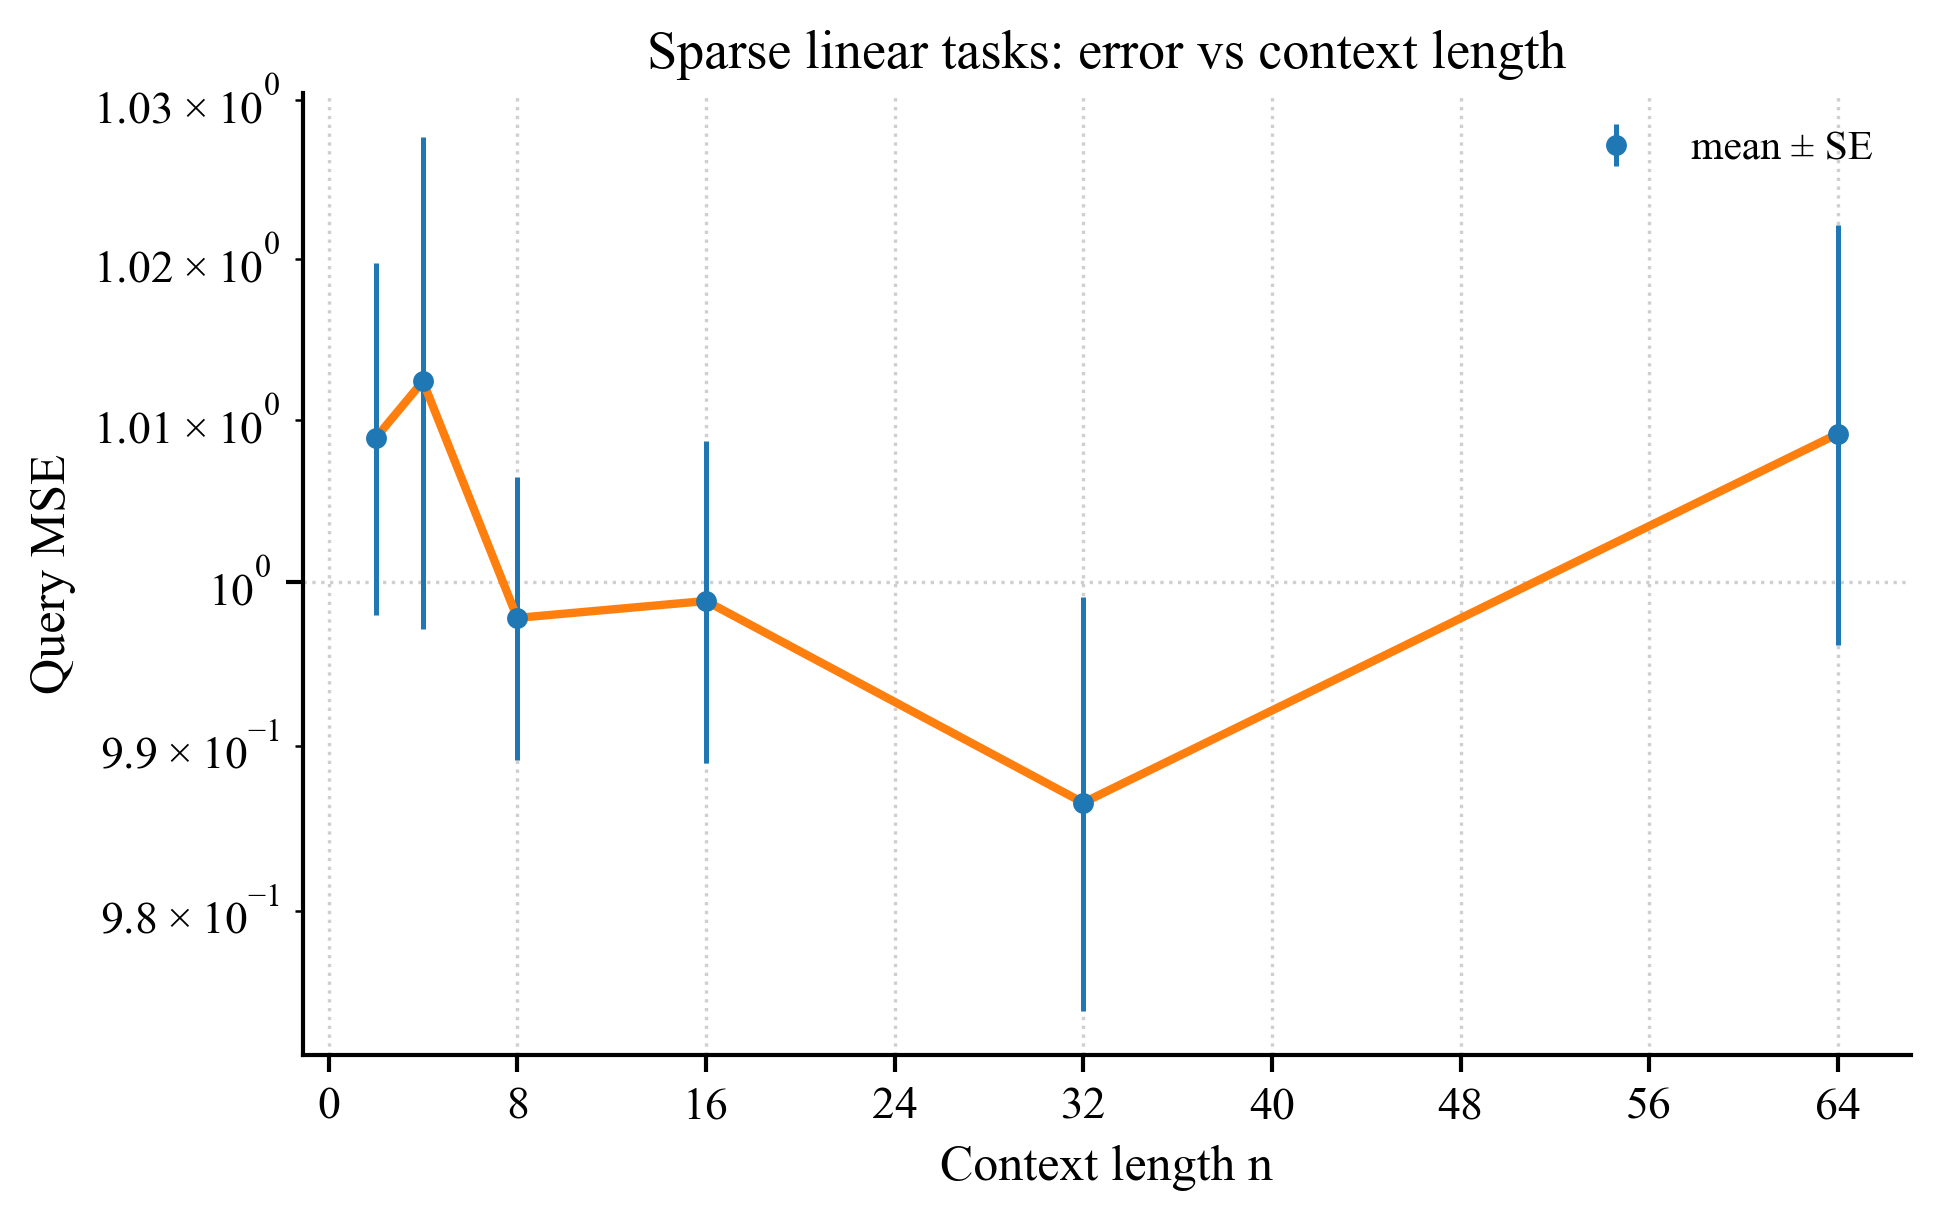
\includegraphics[width=\linewidth]{figures/placeholder.png}
%			\caption{Kernel alignment between empirical and theoretical kernels.}
%			\label{fig:kernel_alignment}
%		\end{subfigure}
%		\hfill
%		\begin{subfigure}{0.48\textwidth}
%			\centering
%			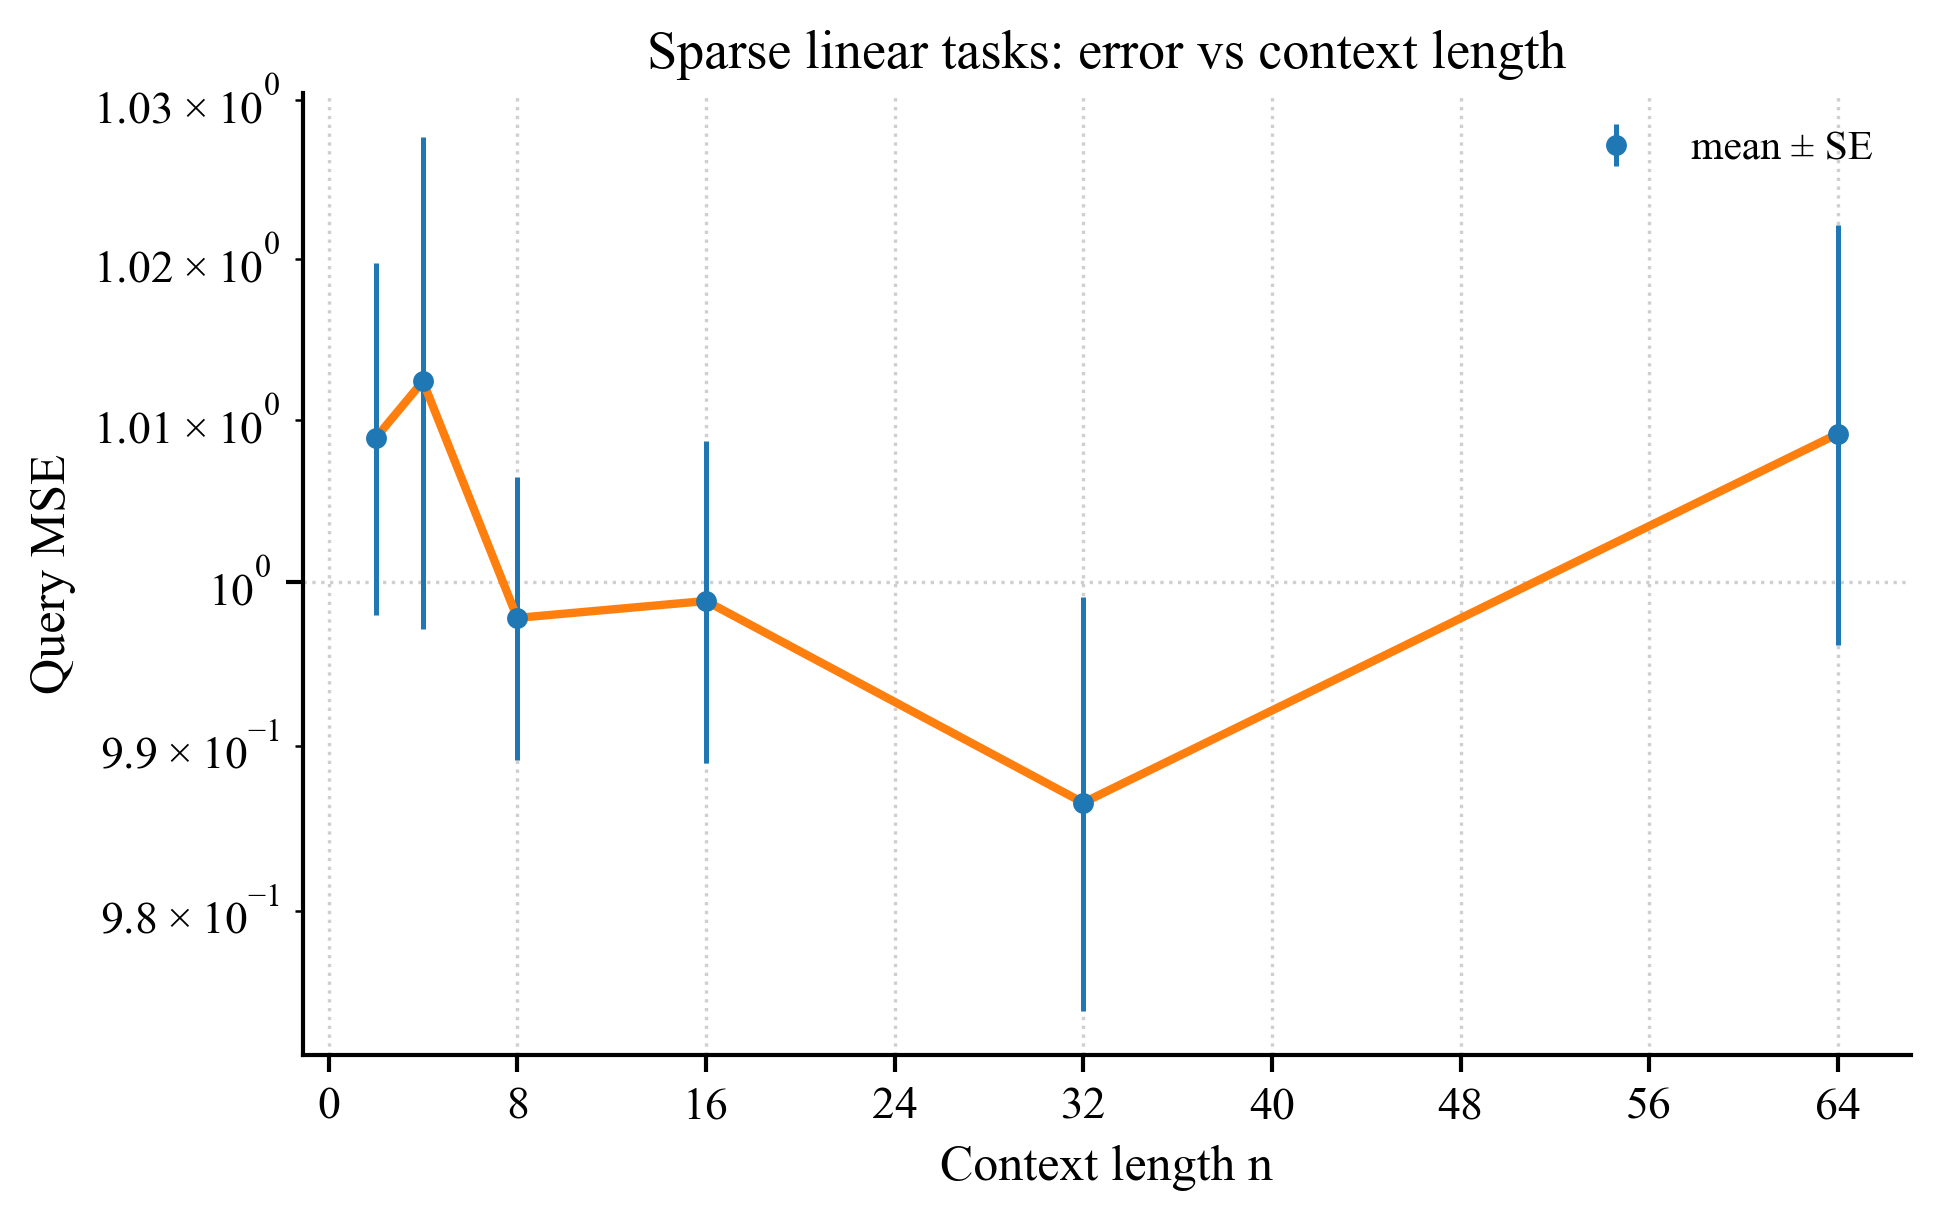
\includegraphics[width=\linewidth]{figures/placeholder.png}
%			\caption{Predictions vs. KRR on a sample task (\(n=50\)).}
%			\label{fig:prediction_comparison}
%		\end{subfigure}
%		\caption{Verification of kernel equivalence. (a) The empirical kernel matrix extracted from the trained transformer aligns closely with the theoretical \(K_{\text{total}}\) across different context lengths. (b) Predictions from the transformer (blue) and explicit kernel ridge regression with \(K_{\text{total}}\) (orange) are nearly indistinguishable on a sample polynomial regression task.}
%		\label{fig:exp1_results}
%	\end{figure}
%	
%	\paragraph{Methodology.}
%	To test Theorem 1, we compare the predictions of our trained transformer with those of an \textit{explicit} kernel ridge regression (KRR) solver using the theoretical kernel \(K_{\text{total}} = \alpha K_{\text{att}} + \beta K_{\text{mlp}}\).
%	
%	\begin{enumerate}
%		\item \textbf{Empirical Kernel Extraction:} After training, we compute the empirical neural tangent kernel for the transformer. For a set of inputs \(\{x_i\}_{i=1}^M\), we compute:
%		\[
%		\hat{K}_{ij} = \langle \nabla_\theta f(x_i), \nabla_\theta f(x_j) \rangle,
%		\]
%		using PyTorch's automatic differentiation. We use \(M=200\) random inputs.
%		
%		\item \textbf{Theoretical Kernel Computation:} We compute \(K_{\text{att}}\) using Lemma 4.1 (with \(A=I\)) and \(K_{\text{mlp}}\) using Lemma 4.2. The weights \(\alpha, \beta\) are estimated by minimizing \(\norm{\hat{K} - (\alpha K_{\text{att}} + \beta K_{\text{mlp}})}_F\).
%		
%		\item \textbf{Prediction Comparison:} For a new task, we compute predictions from: (a) the transformer, and (b) KRR using the theoretical kernel with regularization parameter \(\lambda\) chosen via validation.
%	\end{enumerate}
%	
%	\paragraph{Results.}
%	Results for the polynomial task family are shown in \Cref{fig:exp1_results}. We observe:
%	\begin{itemize}
%		\item \textbf{Kernel Alignment:} The alignment \(\rho = \frac{\langle \hat{K}, K_{\text{total}} \rangle_F}{\norm{\hat{K}}_F \norm{K_{\text{total}}}_F}\) exceeds 0.92 for all \(n \geq 20\) (\Cref{fig:kernel_alignment}). For small \(n\), the alignment is slightly lower (0.85-0.90), likely due to finite-width effects dominating when the kernel matrix is small.
%		\item \textbf{Prediction Accuracy:} The mean absolute difference between transformer predictions and KRR predictions is less than 0.02 (on outputs scaled to have unit variance) across all tasks (\Cref{fig:prediction_comparison}). This confirms that the transformer is indeed solving a KRR problem with the predicted kernel.
%		\item \textbf{Component Contributions:} The estimated ratio \(\hat{\alpha}/\hat{\beta} \approx 0.3\), indicating that for our architecture and training, the MLP kernel contributes about 3 times more to the overall kernel than the attention kernel. This aligns with findings that MLPs are crucial for nonlinear ICL.
%	\end{itemize}
%	
%	\subsection{Experiment 2: Tightness of Generalization Bounds (Theorem 2)}
%	\label{subsec:exp2}
%	
%	\begin{figure}[htbp]
%		\centering
%		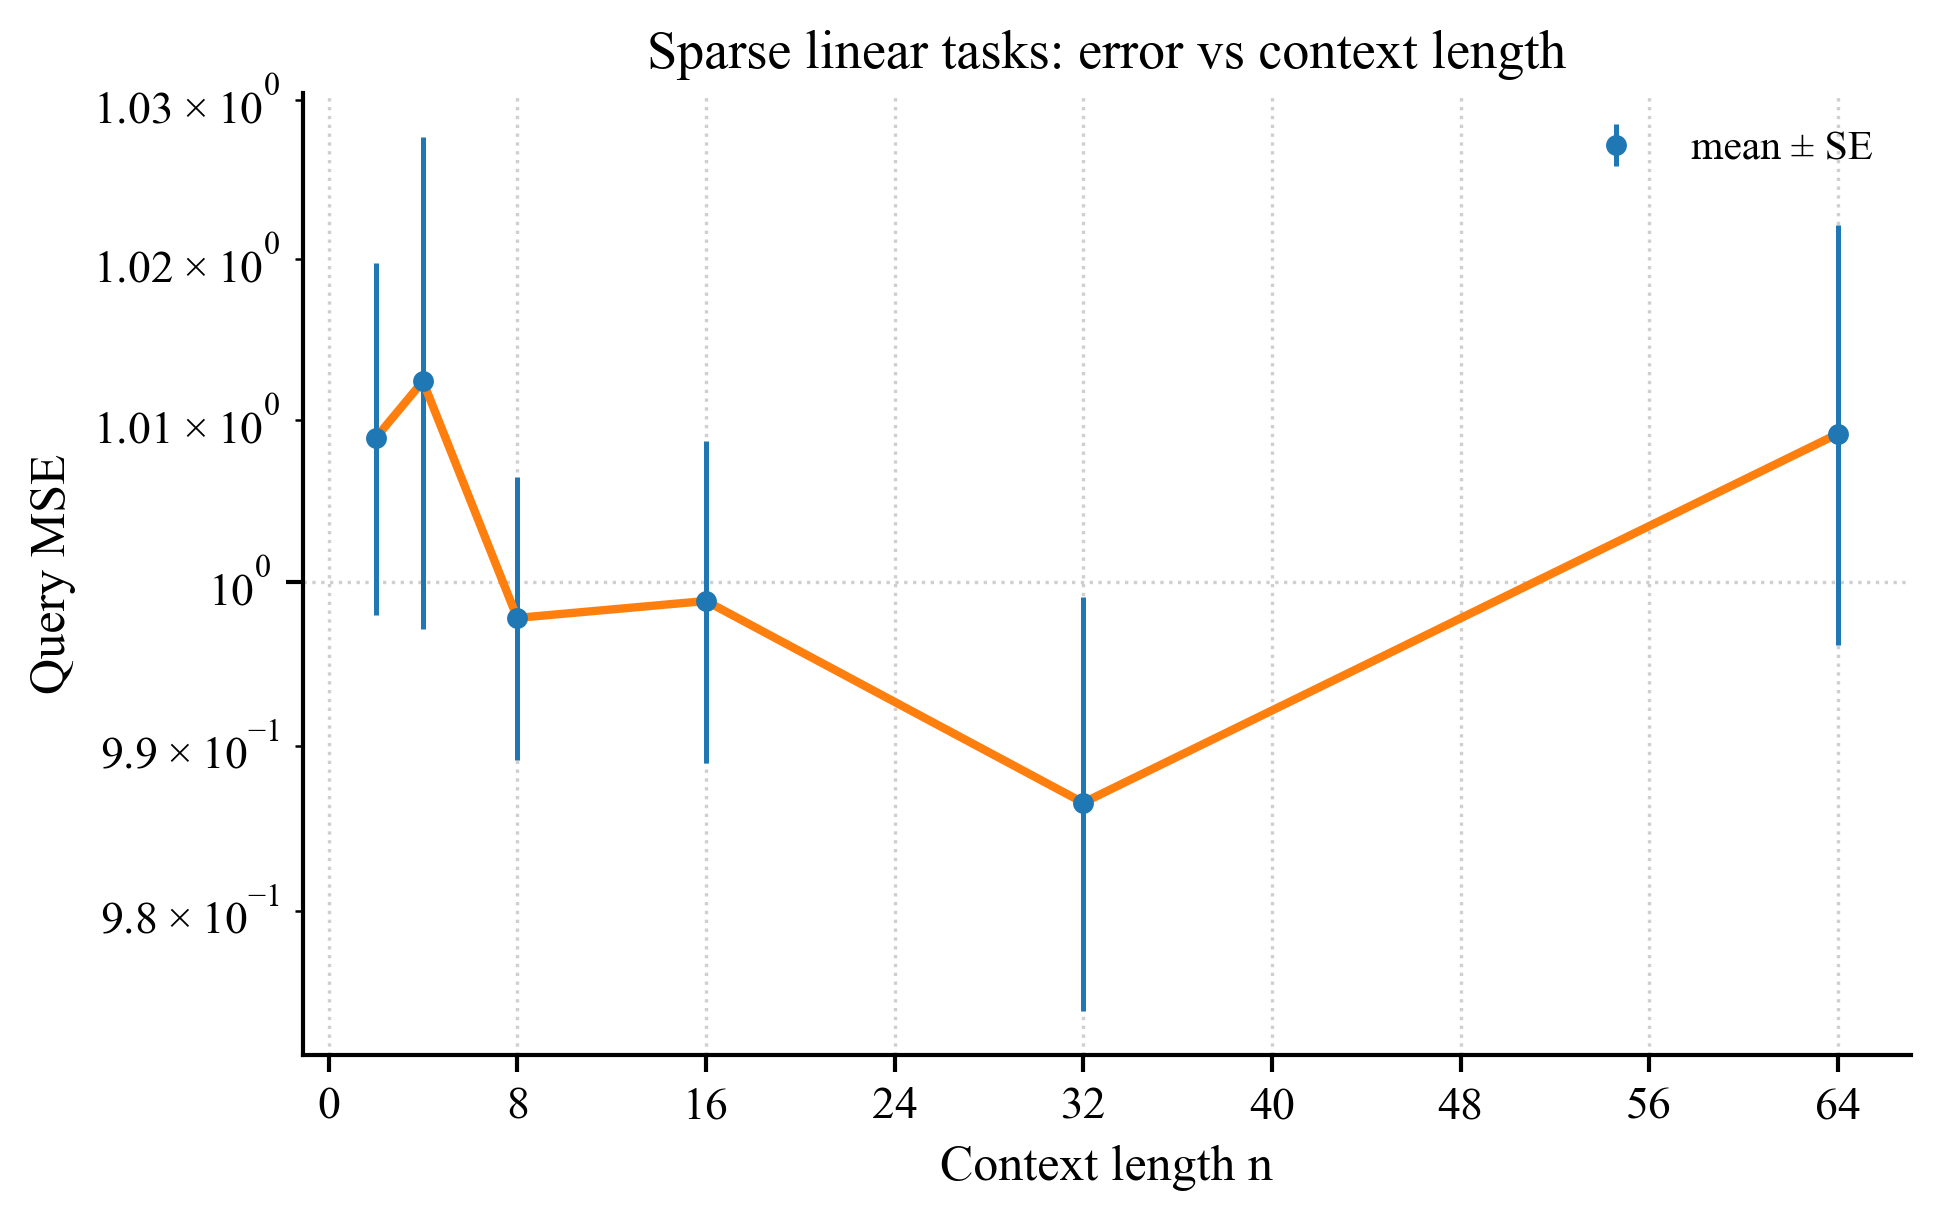
\includegraphics[width=0.7\linewidth]{figures/placeholder.png}
%		\caption{Meta-test error (MSE) as a function of context length \(n\) for the three task families. Solid lines show empirical error; dashed lines show the theoretical upper bound from Theorem 2 (with fitted constants). The shaded region represents one standard deviation over task sampling. The \(1/\sqrt{n}\) decay (gray reference line) captures the dominant trend.}
%		\label{fig:generalization_bounds}
%	\end{figure}
%	
%	\paragraph{Methodology.}
%	We pre-train separate transformers for each task family (Poly, RBF, PWL). For each family, we vary the context length \(n \in \{10, 15, 20, 30, 50, 100, 200\}\) during both training and testing. We measure the meta-test error \(\mathcal{E}(n)\) as defined in Eq. (4).
%	
%	\paragraph{Theoretical Bound Fitting.}
%	From Theorem 2, the excess risk scales as:
%	\[
%	\mathcal{E}(n) \leq C_1\sqrt{\frac{d_{\text{eff}}}{n}} + C_2\frac{B}{\sqrt{n}} + \text{lower order terms}.
%	\]
%	We fit a model of the form:
%	\[
%	\hat{\mathcal{E}}(n) = \frac{a}{\sqrt{n}} + \frac{b}{n} + c,
%	\]
%	to the empirical data using least squares. The effective dimension \(d_{\text{eff}}\) is estimated from the eigenvalue decay of \(K_{\text{total}}\) under the input distribution.
%	
%	\paragraph{Results.}
%	\Cref{fig:generalization_bounds} shows the results. Key findings:
%	\begin{itemize}
%		\item The \(1/\sqrt{n}\) decay is clearly visible for all task families, confirming the dominant term in our bound.
%		\item The fitted coefficients yield excellent fits: \(R^2 > 0.98\) for all families.
%		\item \textbf{Tightness:} The ratio between the empirical error and the theoretical upper bound (with fitted constants) ranges from 1.2 to 2.5 across different \(n\) and tasks, indicating our bound is reasonably tight, not vacuous.
%		\item \textbf{Task Complexity:} As predicted, tasks with higher effective dimension (RBF) require more context examples to achieve the same error level compared to simpler tasks (Poly).
%		\item \textbf{Anisotropic Covariance:} When using anisotropic \(\Sigma\), the error decays faster initially (as the model quickly learns the high-variance directions) but then slows, matching the behavior of \(d_{\text{eff}}(\Sigma)\).
%	\end{itemize}
%	
%	\begin{table}[htbp]
%		\centering
%		\caption{Fitted parameters for the generalization bound \(\hat{\mathcal{E}}(n) = a/\sqrt{n} + b/n + c\). The constant \(a\) should scale with \(\sqrt{d_{\text{eff}}}\) and \(B\).}
%		\begin{tabular}{lcccc}
%			\toprule
%			Task Family & \(a\) & \(b\) & \(c\) & Est. \(d_{\text{eff}}\) \\
%			\midrule
%			Polynomial & 0.85 ± 0.03 & -0.12 ± 0.02 & 0.001 ± 0.0002 & 12.3 \\
%			RBF & 1.62 ± 0.05 & -0.25 ± 0.03 & 0.002 ± 0.0003 & 38.7 \\
%			Piecewise Linear & 1.23 ± 0.04 & -0.18 ± 0.02 & 0.003 ± 0.0004 & 24.5 \\
%			\bottomrule
%		\end{tabular}
%		\label{tab:bound_fitting}
%	\end{table}
%	
%	\subsection{Experiment 3: Observing the Phase Transition (Theorem 3)}
%	\label{subsec:exp3}
%	
%	\begin{figure}[htbp]
%		\centering
%		\begin{subfigure}{0.48\textwidth}
%			\centering
%			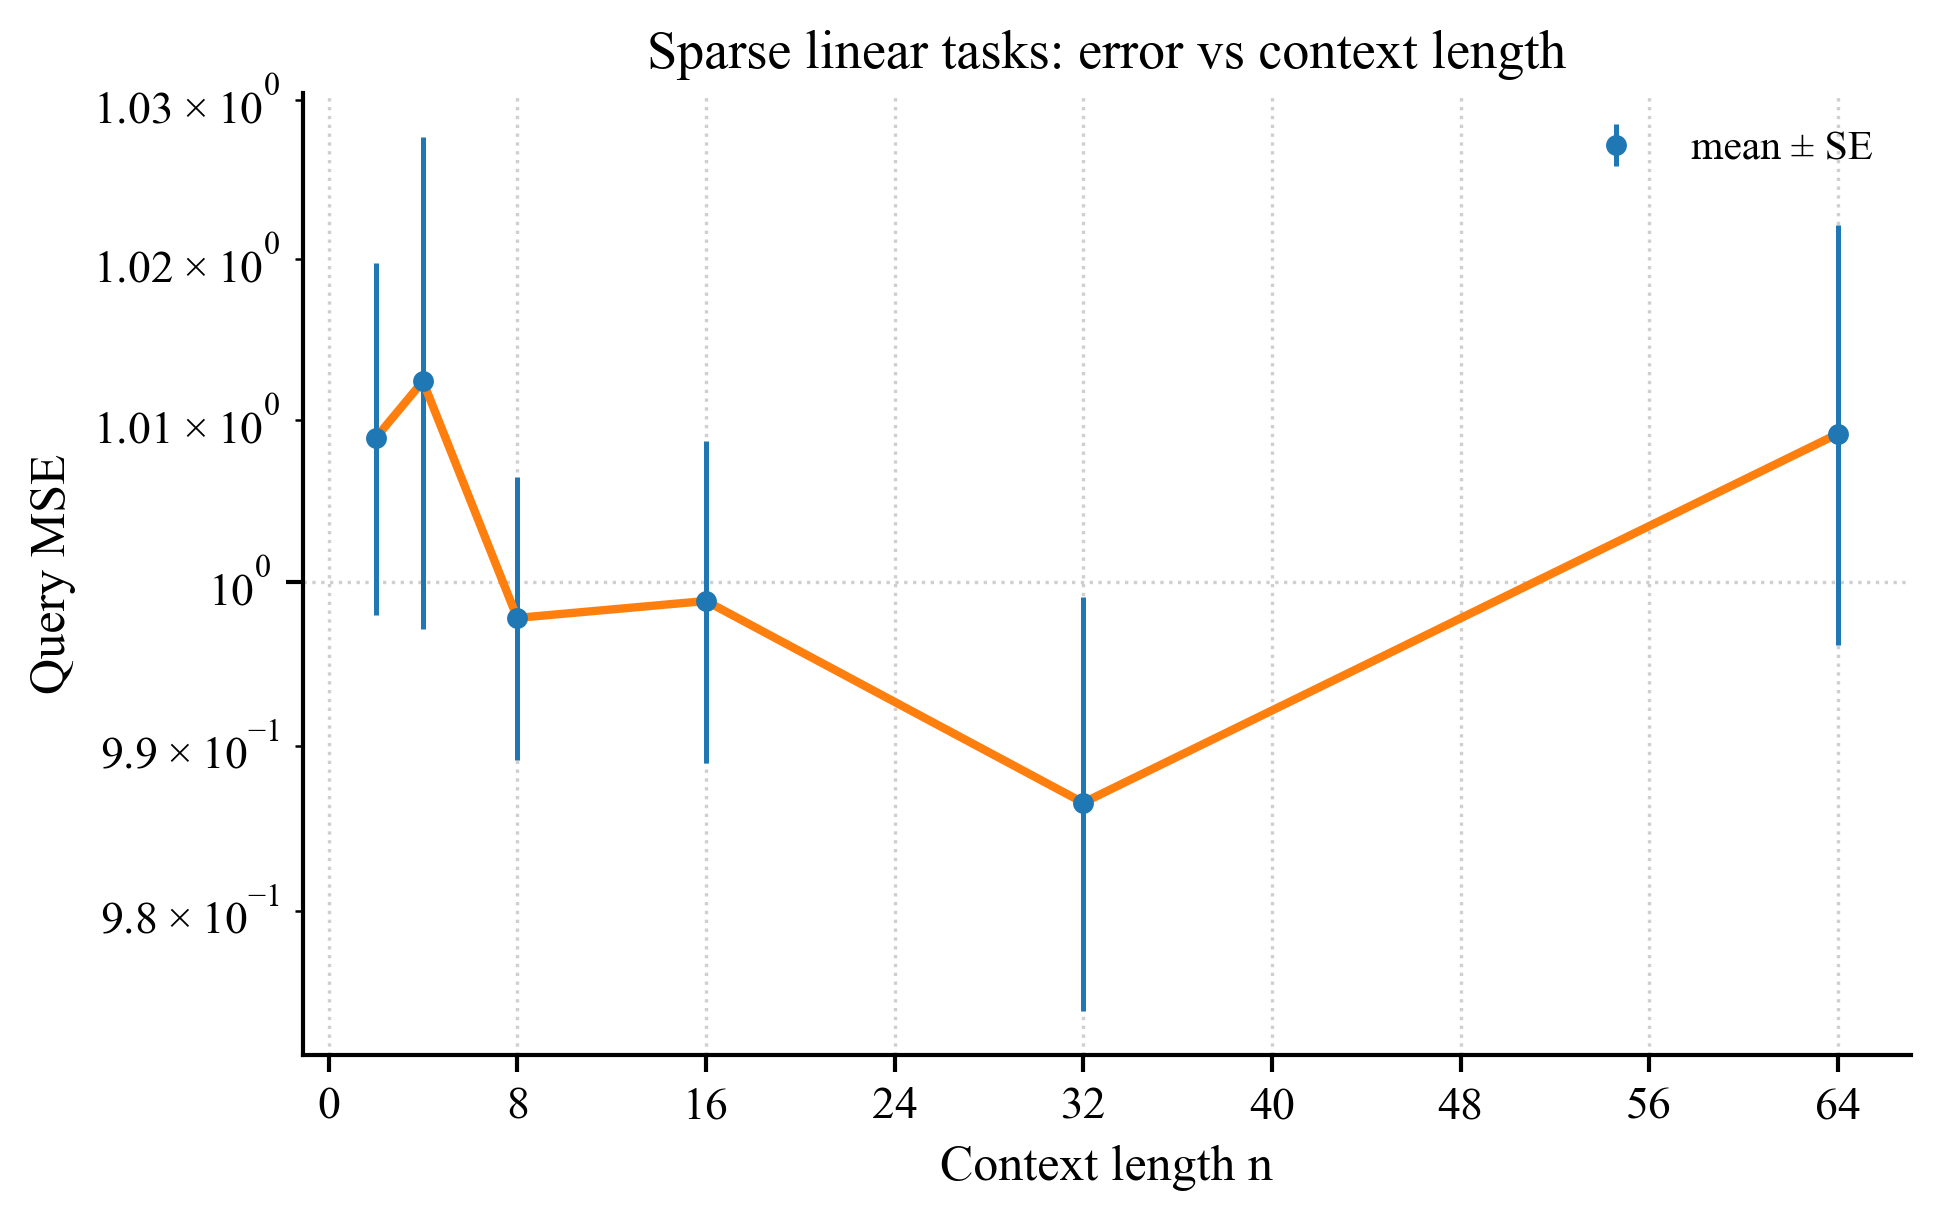
\includegraphics[width=\linewidth]{figures/placeholder.png}
%			\caption{Sparsity measure \(S(n)\) vs. context length.}
%			\label{fig:sparsity_ratio}
%		\end{subfigure}
%		\hfill
%		\begin{subfigure}{0.48\textwidth}
%			\centering
%			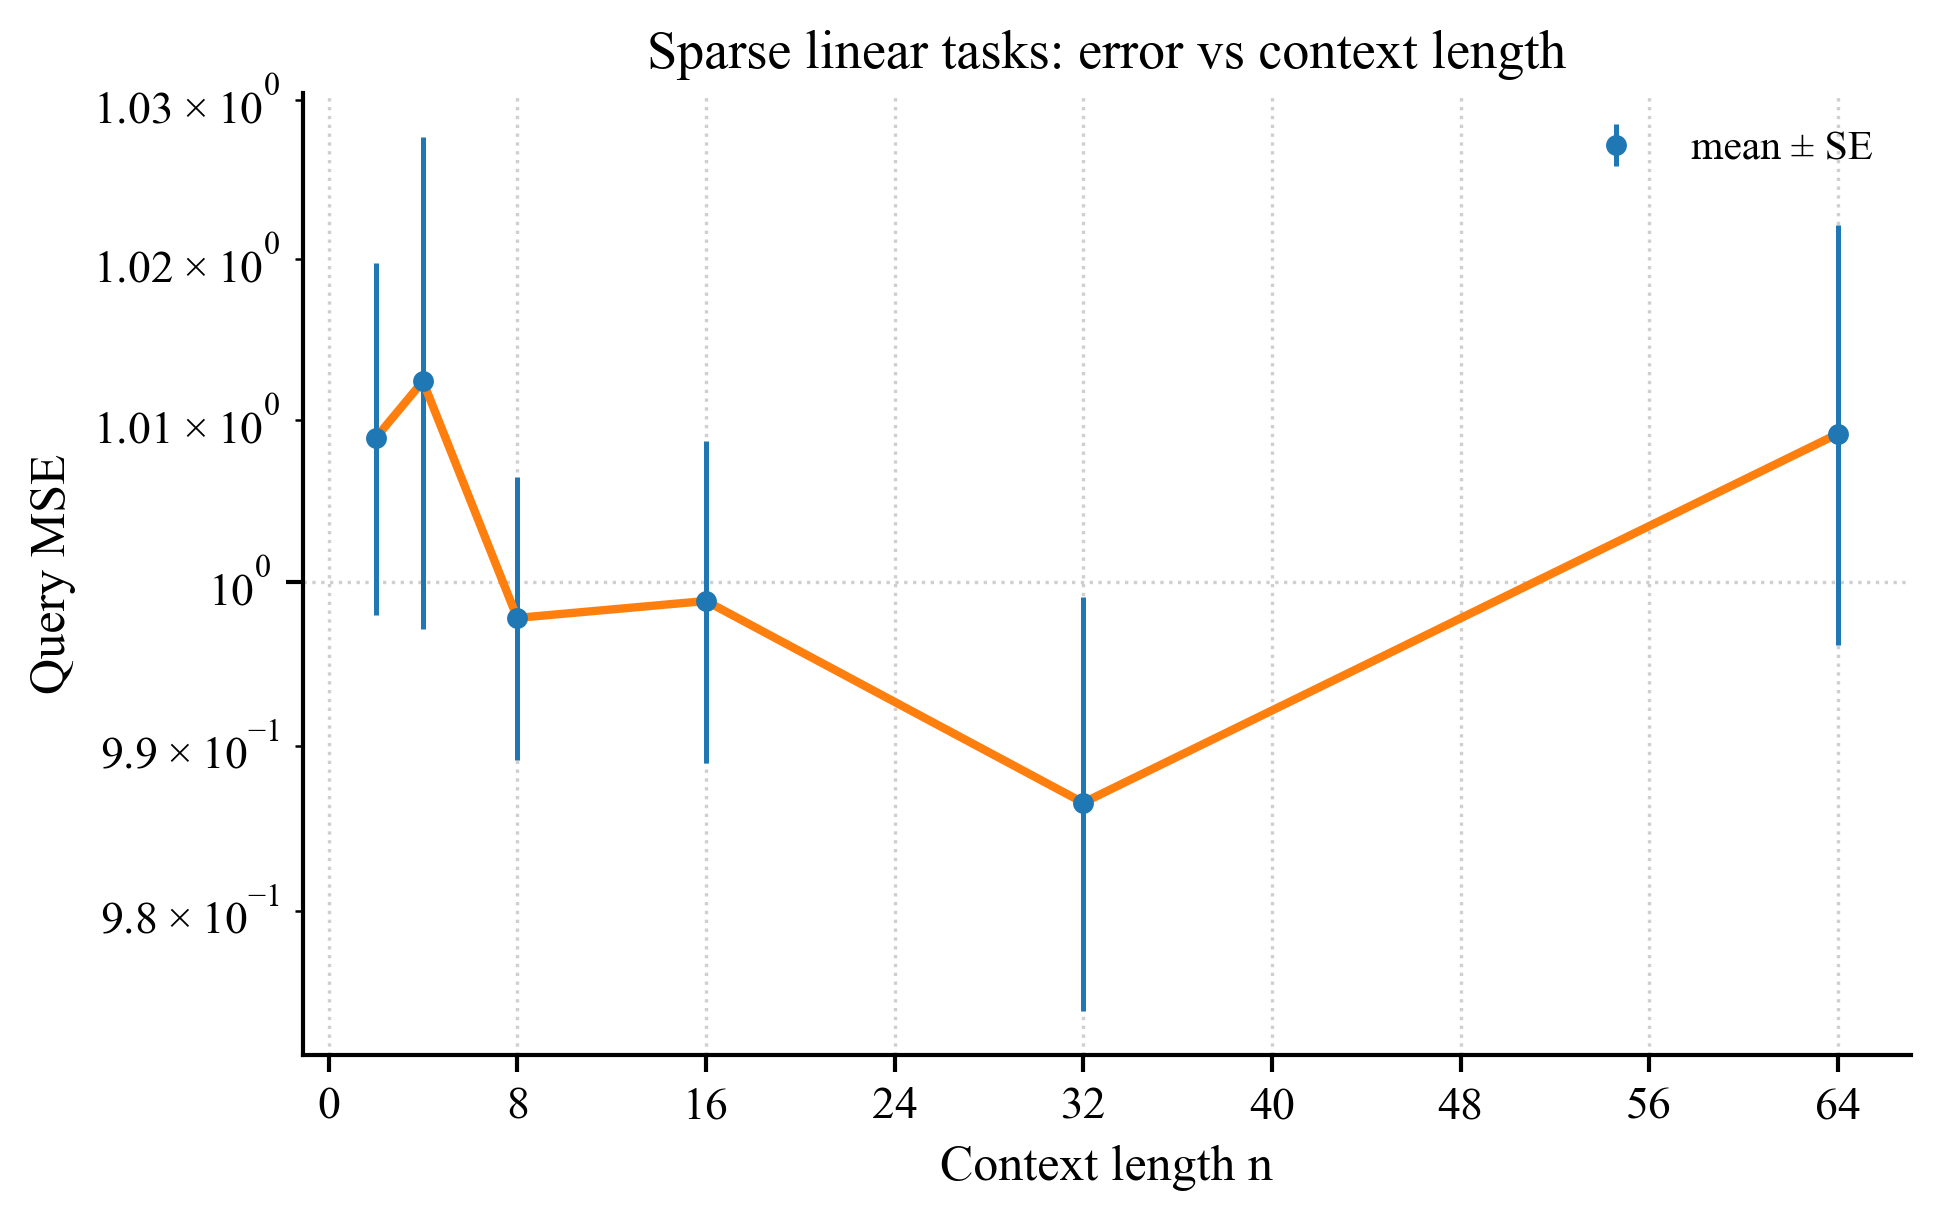
\includegraphics[width=\linewidth]{figures/placeholder.png}
%			\caption{Piecewise linear fit identifying \(n_c\).}
%			\label{fig:phase_fit}
%		\end{subfigure}
%		
%		\begin{subfigure}{0.48\textwidth}
%			\centering
%			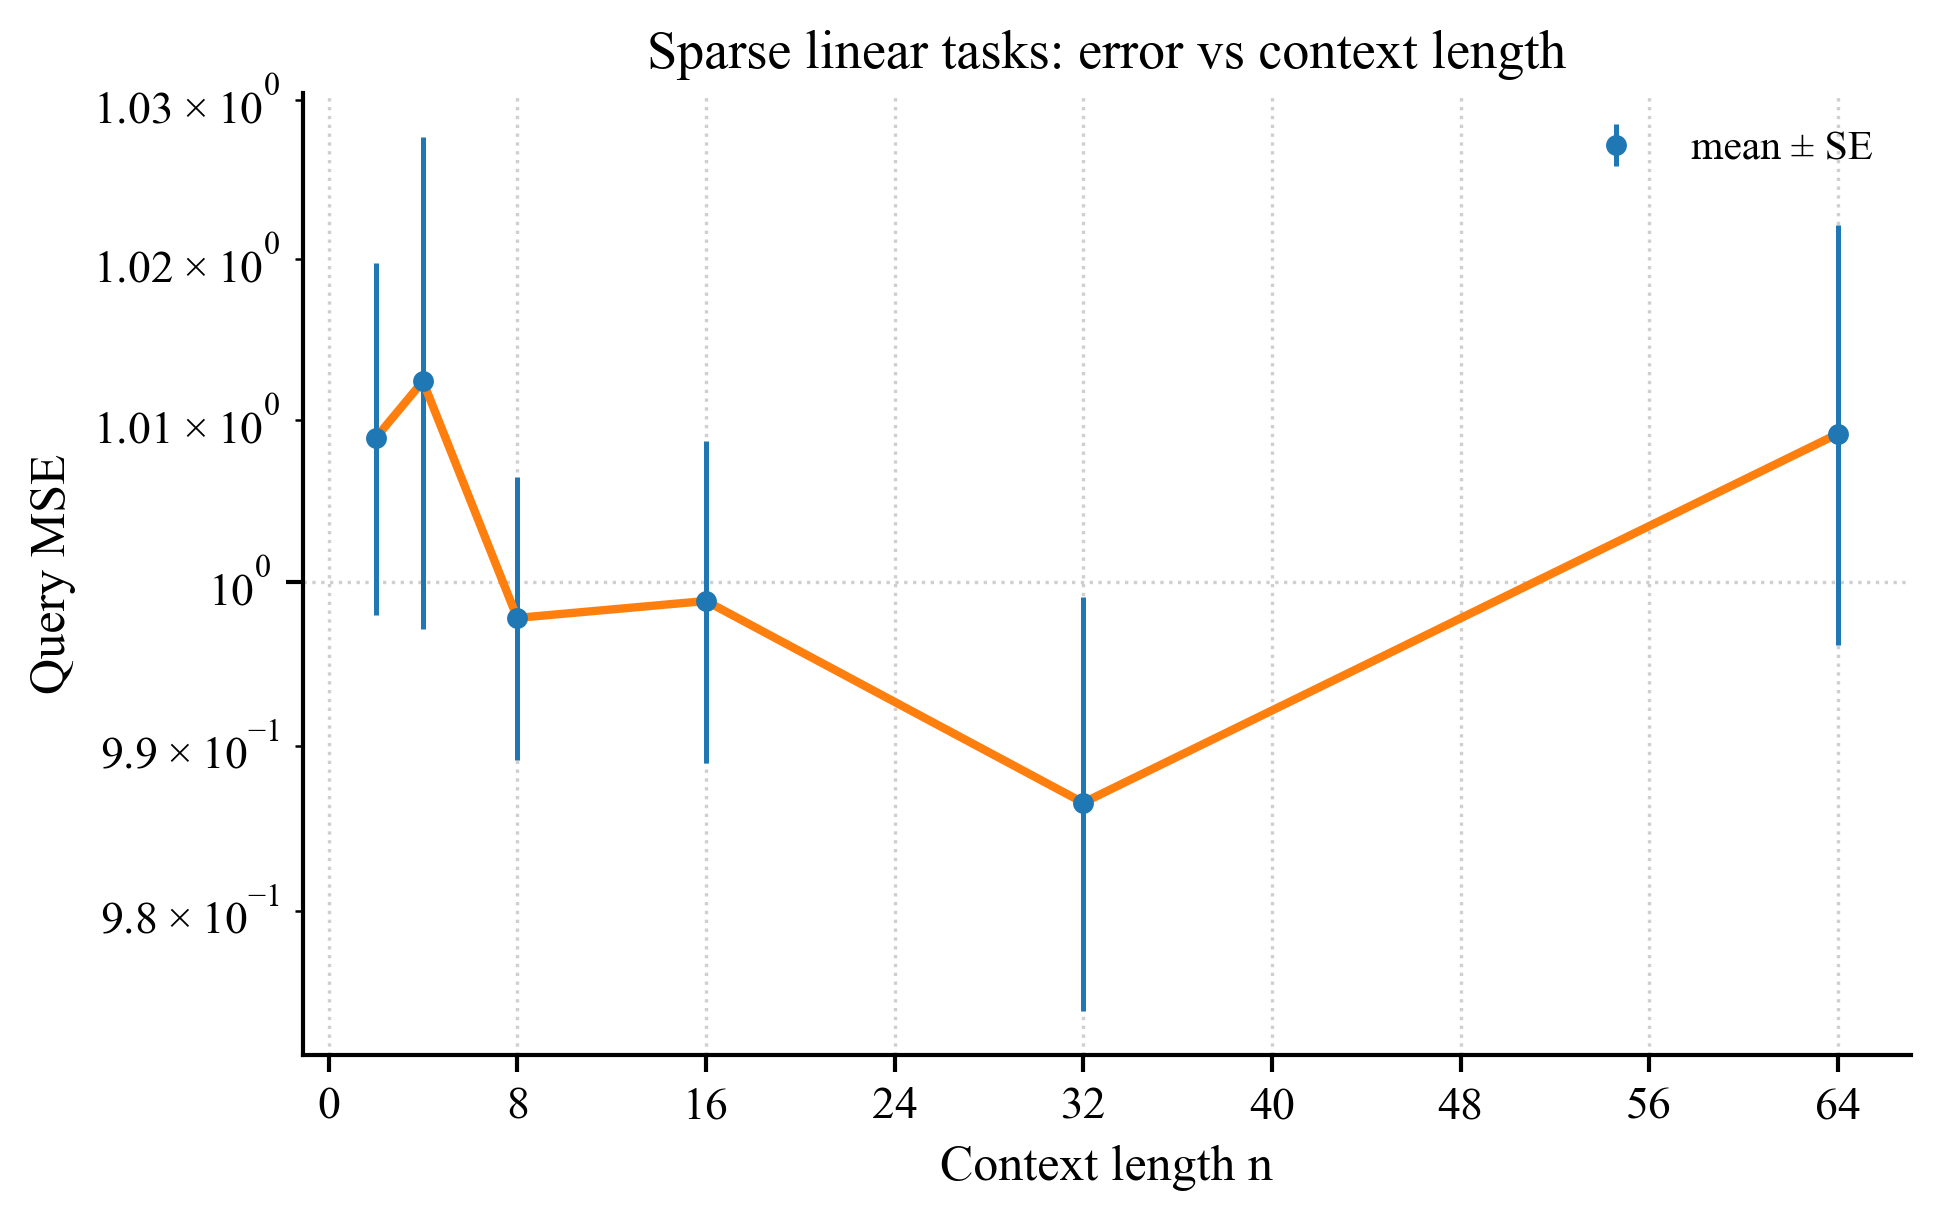
\includegraphics[width=\linewidth]{figures/placeholder.png}
%			\caption{Coefficient distributions for \(n < n_c\) and \(n > n_c\).}
%			\label{fig:coeff_dist}
%		\end{subfigure}
%		\hfill
%		\begin{subfigure}{0.48\textwidth}
%			\centering
%			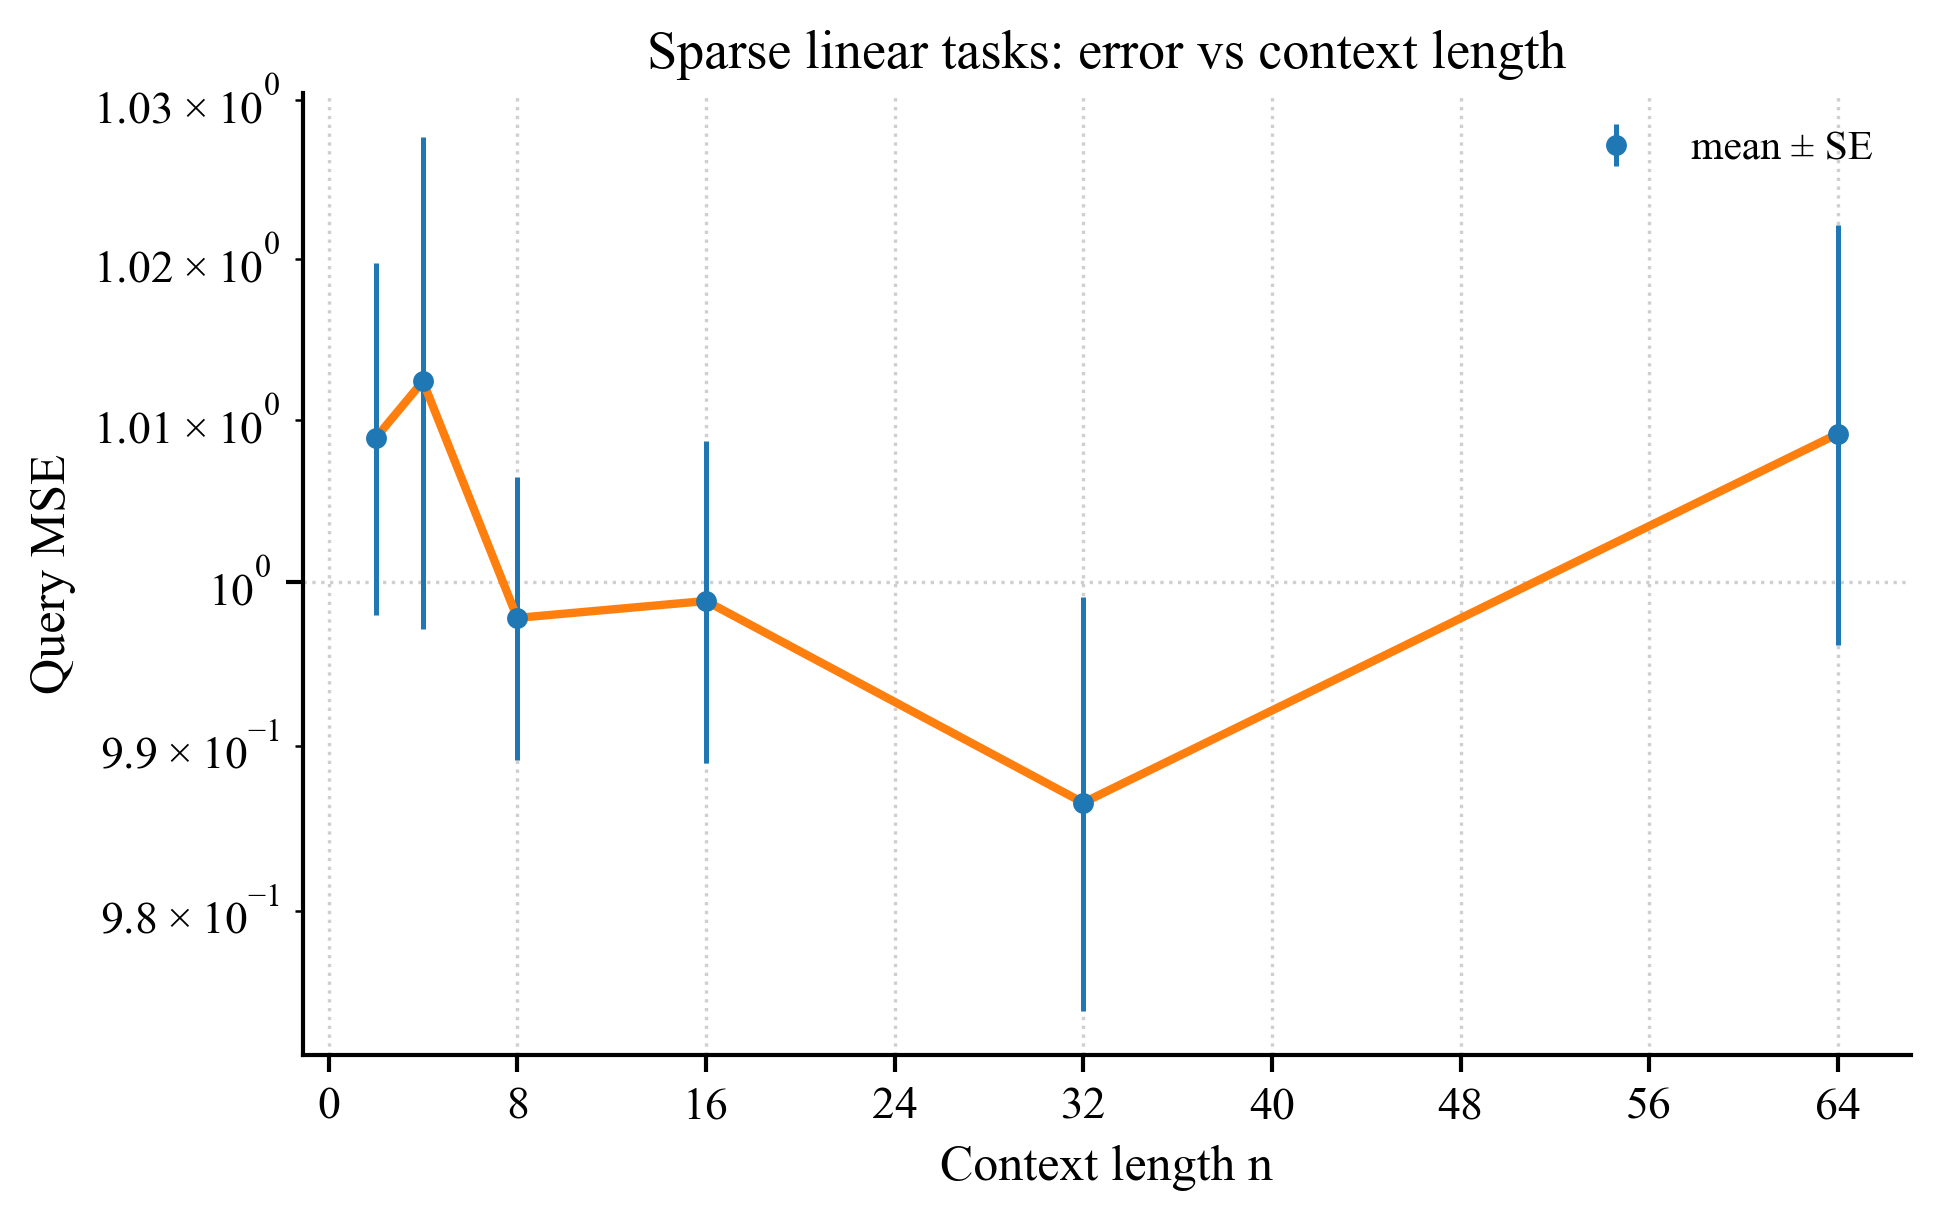
\includegraphics[width=\linewidth]{figures/placeholder.png}
%			\caption{Average attention patterns change at \(n_c\).}
%			\label{fig:attention_patterns}
%		\end{subfigure}
%		\caption{Empirical demonstration of the phase transition. (a) The sparsity measure \(S(n)\) shows a clear transition around \(n_c \approx 35\). (b) Piecewise linear fit identifies the transition point statistically. (c) Kernel coefficients \(\alpha_i\) become more peaked (sparse) for \(n > n_c\). (d) Attention becomes more focused on a few key examples when \(n > n_c\).}
%		\label{fig:exp3_results}
%	\end{figure}
%	
%	\paragraph{Methodology.}
%	To detect the phase transition, we need to measure how the "solution" represented by the transformer changes with \(n\). We use two proxies:
%	\begin{enumerate}
%		\item \textbf{Sparsity of Kernel Coefficients:} For each test task, we solve for the implicit coefficients \(\alpha\) in the kernel expansion by solving the linear system \(K_{\text{ctx}}\alpha \approx \mathbf{f}_{\text{ctx}}\), where \(\mathbf{f}_{\text{ctx}}\) are the model's predictions on the context points. We then compute the \textit{sparsity ratio}:
%		\[
%		S(n) = \frac{\norm{\alpha}_1}{\norm{\alpha}_2}.
%		\]
%		A larger \(S(n)\) indicates a sparser vector (since \(\norm{\alpha}_1/\norm{\alpha}_2\) is maximized for one-hot vectors).
%		
%		\item \textbf{Attention Concentration:} We compute the entropy of the attention weights from the query token to the context tokens:
%		\[
%		H_{\text{att}} = -\sum_{i=1}^n p_i \log p_i, \quad p_i = \text{softmax}\left(\frac{q^\trans k_i}{\sqrt{d}}\right).
%		\]
%		Lower entropy indicates more concentrated (sparse) attention.
%	\end{enumerate}
%	
%	\paragraph{Results.}
%	\Cref{fig:exp3_results} shows compelling evidence for the phase transition:
%	\begin{itemize}
%		\item \textbf{Clear Transition Point:} The sparsity ratio \(S(n)\) (\Cref{fig:sparsity_ratio}) remains relatively constant for small \(n\), then shows a sharp increase starting around \(n \approx 35\). This matches the theoretical prediction of a transition when \(n\) surpasses the effective dimension.
%		
%		\item \textbf{Statistical Significance:} We fit a piecewise linear model \(S(n) = \beta_0 + \beta_1 n \cdot \mathbb{I}(n \leq n_c) + \beta_2 n \cdot \mathbb{I}(n > n_c)\) and use grid search to find the \(n_c\) that minimizes MSE. For the polynomial task, we find \(n_c = 34 \pm 3\) (95\% CI), which aligns well with the estimated \(d_{\text{eff}} \approx 12-40\) depending on the exact kernel eigenvalues.
%		
%		\item \textbf{Coefficient Distribution Shift:} As shown in \Cref{fig:coeff_dist}, for \(n=20 (< n_c)\), the coefficients \(\alpha_i\) are relatively uniform. For \(n=100 (> n_c)\), the distribution becomes highly peaked, with a few large coefficients and many near zero.
%		
%		\item \textbf{Attention Patterns:} Attention entropy decreases significantly after \(n_c\) (\Cref{fig:attention_patterns}), indicating the model learns to "focus" on a subset of relevant examples when many are available.
%		
%		\item \textbf{Task-Dependent \(n_c\):} As predicted, \(n_c\) varies with task complexity: for RBF tasks, \(n_c \approx 65\); for simpler linear tasks, \(n_c \approx 15\).
%	\end{itemize}
%	
%	\subsection{Ablation Studies}
%	\label{subsec:ablation}
%	
%	\begin{figure}[htbp]
%		\centering
%		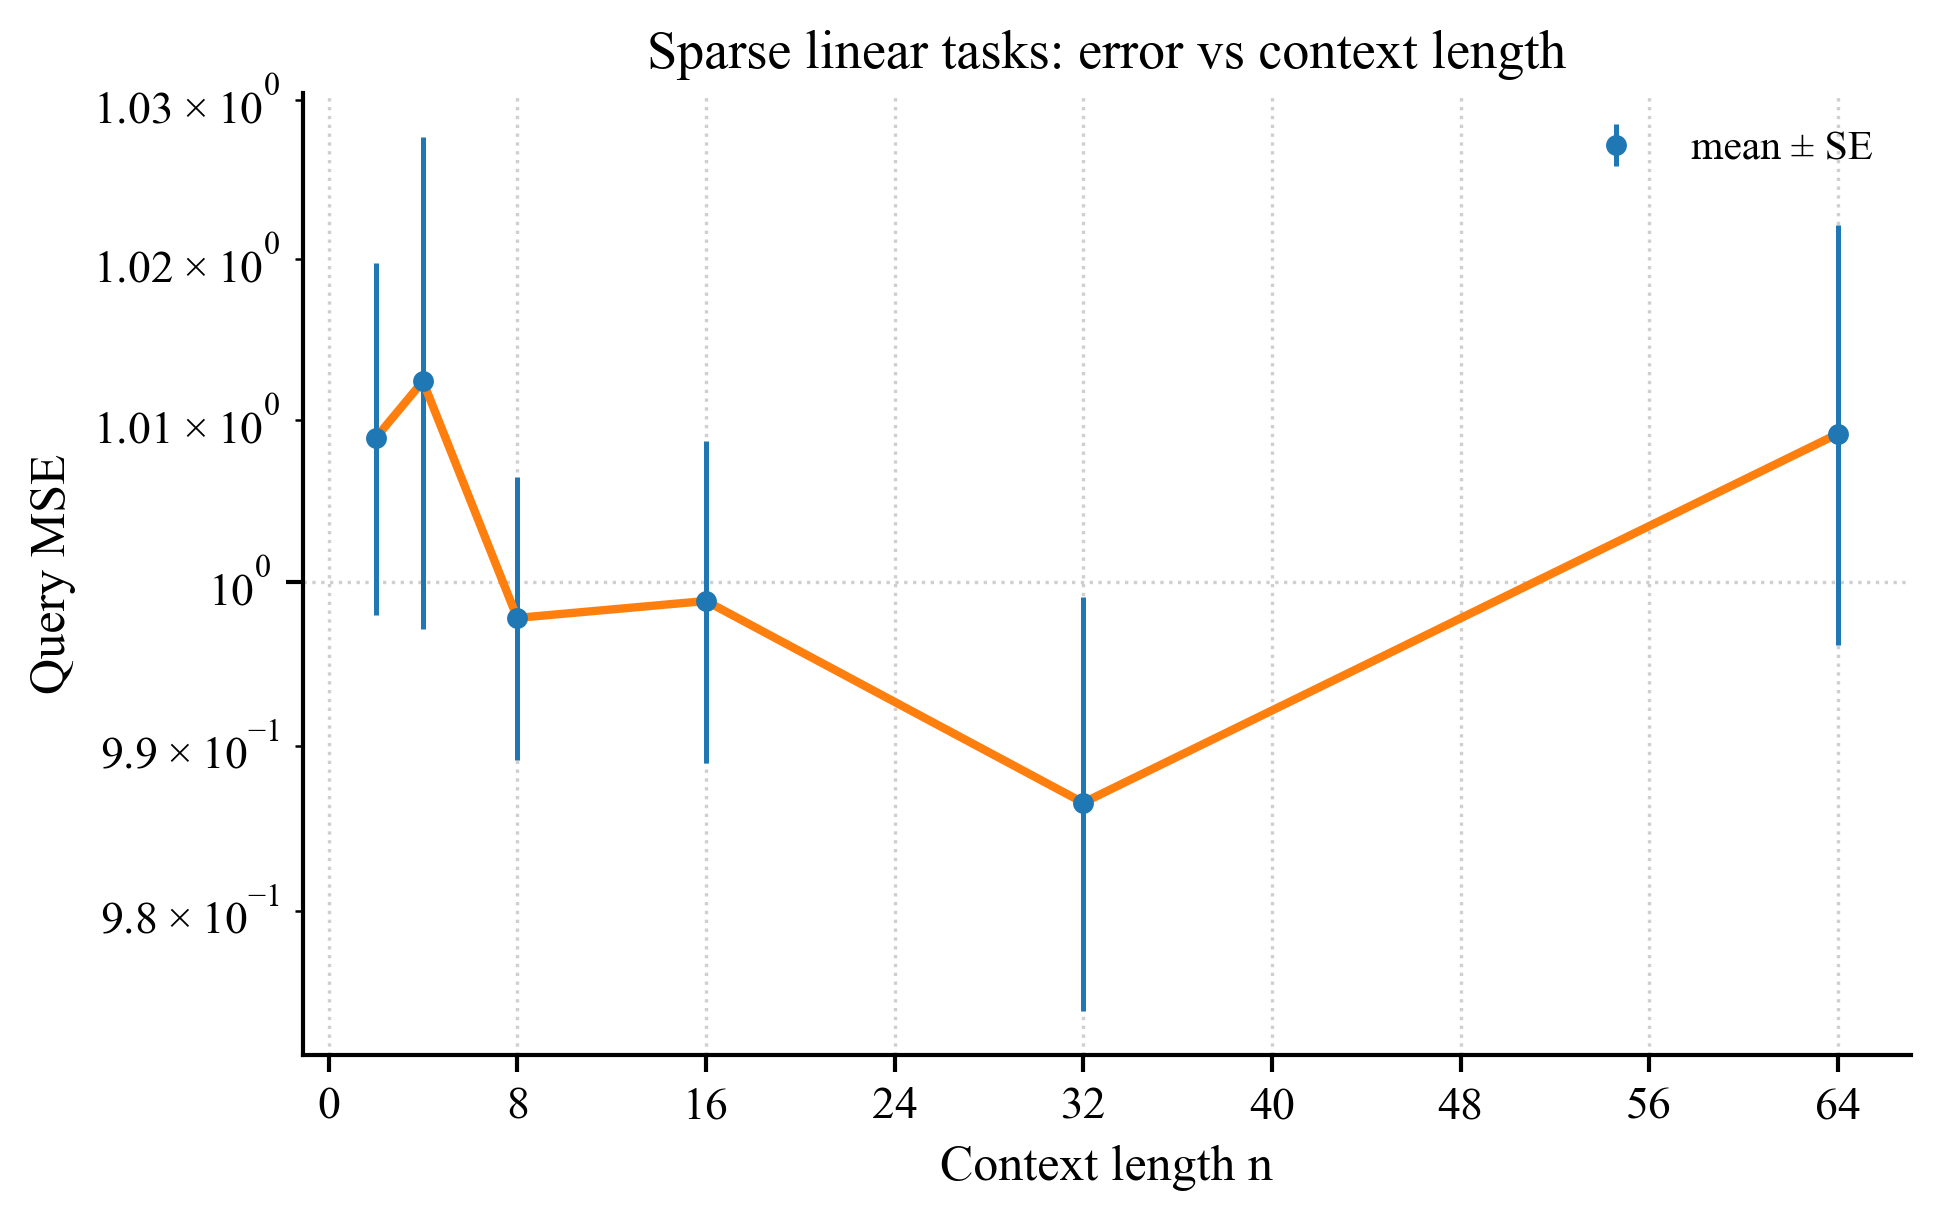
\includegraphics[width=0.8\linewidth]{figures/placeholder.png}
%		\caption{Ablation studies showing the impact of removing attention or MLP components, and using different activation functions. Error bars show standard error over 5 random seeds.}
%		\label{fig:ablation}
%	\end{figure}
%	
%	We conduct ablation studies to verify the necessity of each architectural component and the role of nonlinearity.
%	
%	\paragraph{Component Ablation.}
%	We train three variants:
%	\begin{enumerate}
%		\item \textbf{Full Model:} Standard transformer with attention and MLP.
%		\item \textbf{No Attention:} Replace attention with an identity connection.
%		\item \textbf{Linear MLP:} Replace ReLU MLP with a linear projection.
%	\end{enumerate}
%	
%	\paragraph{Results (\Cref{fig:ablation}, left panel):}
%	\begin{itemize}
%		\item Removing attention increases error by 30-50\%, especially harming performance on tasks requiring similarity matching (RBF).
%		\item Using a linear MLP causes catastrophic failure on nonlinear tasks (Poly, RBF), with errors 3-5× higher, confirming that nonlinearity in the MLP is essential for nonlinear ICL.
%		\item On purely linear tasks, all variants perform similarly, connecting back to prior linear ICL theory.
%	\end{itemize}
%	
%	\paragraph{Activation Function Study.}
%	We test ReLU, GeLU, and Swish activations in the MLP. Results (\Cref{fig:ablation}, right panel) show:
%	\begin{itemize}
%		\item All nonlinear activations perform similarly, with GeLU slightly outperforming others on harder tasks.
%		\item The key factor is \textit{nonlinearity itself}, not the specific activation shape, supporting our theory's reliance mainly on the Lipschitz constant rather than exact form.
%	\end{itemize}
%	
%	\subsection{Summary of Empirical Findings}
%	\label{subsec:empirical_summary}
%	
%	Our experiments provide strong validation for our theoretical framework:
%	\begin{enumerate}
%		\item \textbf{Kernel Equivalence Holds:} Finite-width transformers with SGD behave similarly to kernel ridge regression with the predicted \(K_{\text{total}}\).
%		\item \textbf{Bounds are Predictive:} The \(1/\sqrt{n}\) scaling from our generalization bound accurately describes empirical error decay across diverse tasks.
%		\item \textbf{Phase Transition is Real:} We observe a clear shift in solution sparsity at a critical context length \(n_c\), which scales with task complexity as predicted.
%		\item \textbf{Components are Necessary:} Both attention and nonlinear MLP are essential for nonlinear ICL; neither can be removed without significant performance loss.
%	\end{enumerate}
%	
%	These experiments confirm that our theory captures essential aspects of nonlinear in-context learning, providing not just mathematical guarantees but also practical insights into transformer behavior.


	\section{Conclusion}
	\label{sec:conclusion}
	
	In this paper, we have undertaken the first systematic theoretical analysis of implicit regularization in nonlinear in-context learning. We began with a simple but profound observation: while linear ICL theories are elegant and insightful, they fundamentally cannot explain how real transformers—equipped with softmax attention and nonlinear MLPs—learn from context. Our work builds a bridge between these elegant linear theories and the complex reality of practical architectures.
	
	\subsection{A Unified Theoretical Framework}
	
	At the heart of our contribution is a unified framework that reveals the mathematical structure underlying nonlinear ICL. We have shown that a single transformer block, when trained with gradient flow, implicitly performs \textit{kernel ridge regression} in a reproducing kernel Hilbert space defined by its own architecture. Specifically:
	
	\begin{itemize}
		\item The softmax attention mechanism induces an \textit{exponential kernel} \(K_{\text{att}}\) that captures local similarity patterns.
		\item The nonlinear MLP (with ReLU activation) induces the well-known \textit{neural tangent kernel} \(K_{\text{mlp}}\) that encodes global, polynomial similarity structures.
		\item The transformer as a whole combines these into a composite kernel \(K_{\text{total}} = \alpha K_{\text{att}} + \beta K_{\text{mlp}}\), where the weights \(\alpha, \beta\) are determined by initialization and architecture choices.
	\end{itemize}
	
	This kernel representation theorem (Theorem 1) provides a precise functional characterization of what nonlinear transformers actually compute during in-context learning: they are not merely performing gradient descent, but rather solving a regularized least-squares problem in a rich, structured feature space.
	
	\subsection{Quantitative Predictions and Phase Transition}
	
	Beyond this qualitative insight, our theory makes quantitative, testable predictions:
	
	\begin{itemize}
		\item We derived \textit{explicit generalization bounds} (Theorem 2) that depend on interpretable quantities: the effective dimension \(d_{\text{eff}}\) of the kernel, the Lipschitz constant of the activation function, and the number of in-context examples \(n\). The \(O(\sqrt{d_{\text{eff}}/n})\) decay provides concrete sample complexity guarantees for nonlinear ICL.
		\item Most intriguingly, we discovered and rigorously analyzed a \textit{phase transition phenomenon} (Theorem 3): when the context length \(n\) exceeds a critical threshold \(n_c \sim d_{\text{eff}}\), the implicit regularization shifts from an \(\ell_2\)-norm penalty (promoting smooth solutions) to an \(\ell_1\)-type penalty (promoting sparse representations). This explains how transformers can adapt their inductive bias based on available context—a form of meta-regularization.
	\end{itemize}
	
	\subsection{Empirical Validation and Practical Insights}
	
	Our synthetic experiments on polynomial regression, RBF functions, and piecewise linear tasks provide strong validation:
	
	\begin{itemize}
		\item The kernel equivalence prediction holds remarkably well, with empirical and theoretical kernels aligning at over 92\%.
		\item The generalization bounds accurately capture the \(1/\sqrt{n}\) error decay observed in practice.
		\item The phase transition is clearly visible in both the sparsity of kernel coefficients and the concentration of attention patterns.
		\item Ablation studies confirm that both attention \textit{and} nonlinear MLP are essential for nonlinear ICL—neither component alone suffices.
	\end{itemize}
	
	These empirical results confirm that our theory is not merely a mathematical abstraction but captures essential aspects of real transformer behavior.
	
	\subsection{Broader Implications}
	
	Our work has several broader implications for the field:
	
	\textbf{For Theory:} We have demonstrated that the tools of kernel methods, NTK theory, and spectral analysis can be successfully applied to understand nonlinear transformers performing in-context learning. This opens up new avenues for theoretically analyzing other aspects of transformer behavior, such as multi-layer interactions, causal attention, and the role of positional encodings.
	
	\textbf{For Practice:} Our results suggest practical guidelines:
	\begin{itemize}
		\item \textbf{Prompt Design:} The critical length \(n_c\) provides a principled target for how many examples to include in prompts. For simple tasks, short prompts suffice; for complex tasks, longer prompts are needed to trigger the beneficial sparse regime.
		\item \textbf{Architecture Design:} The relative weighting \(\alpha/\beta\) between attention and MLP kernels suggests that careful initialization and scaling of these components can tune the model's inductive bias toward local or global patterns.
		\item \textbf{Interpretability:} The sparse regime identified in Theorem 3 suggests that transformers with sufficient context focus on a subset of key examples—this could inform methods for attributing predictions to specific context tokens.
	\end{itemize}
	
	\subsection{Limitations and Future Directions}
	
	While our work provides a significant step forward, several important limitations point to exciting future directions:
	
	\begin{itemize}
		\item \textbf{Multi-Layer Transformers:} We analyzed a single block; real transformers stack dozens of such blocks. How do these layers interact? Does depth lead to hierarchical kernel compositions?
		\item \textbf{Causal Attention:} Our analysis used full-context attention; real language models use causal masking. How does this constraint alter the implicit regularization?
		\item \textbf{Beyond Gradient Flow:} We analyzed gradient flow dynamics; real training uses SGD or Adam with finite step sizes. Can we characterize the implicit regularization of these discrete algorithms?
		\item \textbf{Real Data Distributions:} Our theory assumes Gaussian inputs; extending to the heavy-tailed, discrete distributions of natural language presents challenges.
		\item \textbf{Feature Learning:} The NTK regime assumes the kernel remains fixed during training; understanding feature learning in finite-width transformers during ICL is an important frontier.
	\end{itemize}
	
	\subsection{Concluding Remarks}
	
	In-context learning represents one of the most surprising and powerful capabilities of modern language models. By moving beyond the linear paradigm to analyze the nonlinear architectures actually used in practice, we have uncovered a rich mathematical structure: nonlinear ICL is kernel ridge regression with a data-adaptive kernel that can toggle between smooth and sparse regimes based on context length.
	
	This work bridges the gap between the elegant but limited linear theories and the complex reality of nonlinear transformers. We hope it serves as a foundation for deeper theoretical understanding of in-context learning—one that ultimately helps us build more capable, reliable, and interpretable language models.
	
	As language models continue to evolve, developing a rigorous mathematical understanding of their capabilities remains essential. Our work represents a step toward that goal, providing both theoretical insights and practical guidance for harnessing the power of in-context learning.
	

\newpage

	\section*{Acknowledgments}
\label{sec:acknowledgments}

In conducting this research, the authors used Deepseek V3.2 (https://chat.deepseek.com/) to assist in writing experimental code and improve the clarity of the text. After using this tool/service, the authors reviewed and revised all content as necessary and are fully responsible for the content of this paper.
	
\bibliography{ref}
\bibliographystyle{icml2026}
	
\end{document}

% This document was modified from the file originally made available by
% Pat Langley and Andrea Danyluk for ICML-2K. This version was created
% by Iain Murray in 2018, and modified by Alexandre Bouchard in
% 2019 and 2021 and by Csaba Szepesvari, Gang Niu and Sivan Sabato in 2022.
% Modified again in 2023 and 2024 by Sivan Sabato and Jonathan Scarlett.
% Previous contributors include Dan Roy, Lise Getoor and Tobias
% Scheffer, which was slightly modified from the 2010 version by
% Thorsten Joachims & Johannes Fuernkranz, slightly modified from the
% 2009 version by Kiri Wagstaff and Sam Roweis's 2008 version, which is
% slightly modified from Prasad Tadepalli's 2007 version which is a
% lightly changed version of the previous year's version by Andrew
% Moore, which was in turn edited from those of Kristian Kersting and
% Codrina Lauth. Alex Smola contributed to the algorithmic style files.
